% Author: Aigul Mardanova (aigul.mardanova@tu-ilmenau.de)
% https://github.com/aygulmardanova/mt-latex

\documentclass[a4paper,12pt]{report}

%%% Preamble with settings %%%
\usepackage[english, russian]{babel}
\usepackage[utf8]{inputenc}
\usepackage{fancyhdr}
\usepackage{setspace}
\onehalfspacing

\usepackage{lastpage}

\usepackage{geometry}
\geometry{
	a4paper,
%	total={170mm,257mm},
	left=25mm,
	top=25mm,
	right=15mm,
	bottom=25mm
}

\usepackage[compact]{titlesec}
\titleformat{\chapter}
{\normalfont\LARGE\bfseries}{\thechapter}{1em}{}
\titlespacing*{\chapter}{0pt}{-40pt}{30pt}

\let\up\textsuperscript

%% ToDo notes %%
\usepackage{todonotes}

%% Bibliography %%%
\usepackage[square,numbers]{natbib}
\bibliographystyle{unsrt}

\usepackage[nottoc]{tocbibind} % Includes "Bibliography" in contents

\usepackage{fontspec} % XeTeX
\usepackage{xunicode} % Unicode для XeTeX
\usepackage{xltxtra}  % Верхние и нижние индексы
\usepackage{indentfirst} % Indented line after header

%% Listings %%%
\usepackage{listings} % Listings format settings
\usepackage{xcolor}
\usepackage{color, colortbl}

\definecolor{codegreen}{rgb}{0, 0.6, 0}
\definecolor{codegray}{rgb}{0.5, 0.5, 0.5}
\definecolor{codeblue}{rgb}{0.2, 0.2, 0.6}
\definecolor{backgray}{rgb}{0.94,0.94,0.94}
\definecolor{nogray}{rgb}{0.97, 0.97, 0.97}
\definecolor{codepurple}{rgb}{0.58, 0, 0.82}

\lstdefinestyle{code-style-java}{
%	belowcaptionskip=1\baselineskip,			% skip 1 line after listing caption
	xleftmargin=\parindent,
	identifierstyle=\color{blue},
	language=Java,								% the language of the code
	backgroundcolor=\color{backgray}, 			% choose the background color; you must add \usepackage{color} or \usepackage{xcolor}; should come as last argument  
	commentstyle=\color{codegray},				% comment style
	keywordstyle=\color{codeblue}\bfseries,		% keyword style
	numberstyle=\tiny\color{codegray},			% the style that is used for the line-numbers
	stringstyle=\color{codepurple},				% string literal style
	basicstyle=\small\ttfamily\footnotesize,	% Размер и тип шрифта, the size of the fonts that are used for the code
	breakatwhitespace=false,         			% sets if automatic breaks should only happen at whitespace
	breaklines=true,        					% Перенос строк
	captionpos=lt,                    			% sets the caption-position to bottom               
	keepspaces=true,    						% keeps spaces in text, useful for keeping indentation of code (possibly needs columns=flexible)             
	numbers=left,                    			% where to put the line-numbers; possible values are (none, left, right)
	numbersep=5pt,           					% how far the line-numbers are from the code       
	stepnumber=1,                    			% the step between two line-numbers. If it's 1, each line will be numbered
	showspaces=false,           % show spaces everywhere adding particular underscores; it overrides 'showstringspaces'   
	showstringspaces=false,		% underline spaces within strings only		
	showtabs=false,             % show tabs within strings adding particular underscores     
	tabsize=2,					% Размер табуляции, sets default tabsize to 2 spaces
%	frame=single,               % Рамка, adds a frame around the code
%	frame=TB,
	literate={--}{{-{}-}}2,     % Корректно отображать двойной дефис
	literate={---}{{-{}-{}-}}3,  % Корректно отображать тройной дефис
	escapeinside={(*}{*)}
}

\lstdefinestyle{code-style-sql}{
	language=SQL,
	frame=ltrb,
	framesep=5pt,
	basicstyle=\normalsize,
	keywordstyle=\ttfamily\color{OliveGreen},
	identifierstyle=\ttfamily\color{CadetBlue}\bfseries, 
	commentstyle=\color{Brown},
	stringstyle=\ttfamily,
	showstringspaces=true,
	escapeinside={<--}{-->}
}

%\lstset{style=mystyle-pseudo}

% Шрифты, xelatex
\defaultfontfeatures{Ligatures=TeX}
\setmainfont{Times New Roman}
\setmonofont{FreeMono}

%% Graphics & Illustrations %%%%%%%%%%%%%%%%%%%%%%%%%
\usepackage{graphicx}			% Images and additions inserting (to load graphics)
\usepackage{wrapfig}			% integration of graphics with wraping text
%\usepackage{subfig}				% integration of multiple objects within a float
\usepackage{pdfpages}			% PDF inserting, binds a graphic or page (.pdf or .jpg) in the document
\usepackage{float}
\usepackage[section]{placeins}

% Format of labels for figures and tables
\usepackage{chngcntr}
\usepackage{multirow}
\usepackage{array, makecell}
\usepackage{longtable}
\usepackage{booktabs}
\usepackage{array}
\newcolumntype{C}[1]{>{\centering\let\newline\\\arraybackslash\hspace{0pt}}m{#1}}
\usepackage[tableposition=top]{caption}
\usepackage{subcaption}

% Reset the counter for figures, tables in each Chapter
\counterwithin{figure}{section}
\counterwithin{table}{section}

% Format of labels for theorems and definitions
\usepackage{amssymb,amsfonts,amsmath,amsthm,bm} % Maths
\numberwithin{equation}{section} % Formules numbering chapter.number

\theoremstyle{definition}
\newtheorem{definition}{Definition}

\usepackage[yyyymmdd,hhmmss]{datetime}
\usepackage[ruled,vlined]{algorithm2e} 		% algochapter

\renewcommand*{\lstlistlistingname}{List of Listings}


%%%% Joining Algorithms and Listings into one %%%
%\makeatletter
%\AtBeginDocument{%
%	\renewcommand\lstlistlistingname{Algorithms and Listings}
%	\let\c@algocf\c@lstlisting
%}
%\renewcommand{\algocf@list}{lol}%
%\renewcommand*\l@algocf{\@dottedtocline{1}{1.5em}{2.3em}}
%\makeatother
%%%%%%%%

%% HyperRef %%%%%%%%%%%%%%%%%%%%%%%%%%%%%%
% http://www.tug.org/applications/hyperref/manual.html
\usepackage[breaklinks]{hyperref}
\def\UrlBreaks{\do-\do/\do.}
\hypersetup{
    colorlinks, urlcolor={black}, % All links are black and clickable
    linkcolor={black}, citecolor={black}, filecolor={black},
    pdfauthor={Aigul Mardanova},
    pdftitle={Identification of Trajectory Anomalies in Uncertain Spatiotemporal Data}
}

\sloppy             % Избавляемся от переполнений
\hyphenpenalty=1000 % Частота переносов
\clubpenalty=10000  % Запрещаем разрыв страницы после первой строки абзаца
\widowpenalty=10000 % Запрещаем разрыв страницы после последней строки абзаца

% Списки
\usepackage{enumitem}
\setlist[enumerate,itemize]{leftmargin=12.7mm} % Отступы в списках

% Appendix
\usepackage[toc,page]{appendix}

% Page number is bottom-right
\usepackage{fancyhdr}
\pagestyle{fancyplain}
\fancyhf{}
\rhead{\rightmark}
%\rfoot{\thepage}
\fancyfoot[C]{\thepage}
\renewcommand{\headrulewidth}{0.4pt}
\renewcommand{\footrulewidth}{0.4pt}


\usepackage{xassoccnt}
\NewTotalDocumentCounter{totalfigures}
\NewTotalDocumentCounter{totaltables}
\NewTotalDocumentCounter{appendixchapters}
\DeclareAssociatedCounters{figure}{totalfigures}
\DeclareAssociatedCounters{table}{totaltables}

%\renewcommand{\chaptermark}[1]{ \markboth{#1}{} }
%\renewcommand{\sectionmark}[1]{ \markright{#1} }

%% Global Document Information %%%%%%%%%%%%%%%%%%%%%%%%%%%%%%%%%%%%%%%%
% please fill in your personal information
% RUS
\newcommand{\thesistitlerus}{Идентификация аномальных траекторий в неопределенных пространственно-временных данных}
\newcommand{\thesistyperus}{ВЫПУСКНАЯ КВАЛИФИКАЦИОННАЯ РАБОТА}
\newcommand{\authorNamerus}{А. Р. Марданова}
\newcommand{\tutorrus}{д.т.н., проф. И. В. Аникин}
\newcommand{\instituterus}{Компьютерных технологий и защиты информации}
\newcommand{\departmentrus}{Систем информационной безопасности}
\newcommand{\studiesrus}{09.04.01 Информатика и вычислительная техника}
\newcommand{\locationrus}{Казань}
\newcommand{\submissiondaterus}{2020}
\newcommand{\universityrus}{федеральное государственное бюджетное образовательное\\ учреждение высшего образования\\ «Казанский национальный исследовательский\\ технический университет им. А.Н. Туполева-КАИ»\\ (КНИТУ-КАИ)}
%%%%%%%%%%%%%%%%%%%%%%%%%%%%%%%%%%%%%%%%%%%%%%%%%%%%%%%%%%%%%%%%%%%%%%%

%% Настройки для ЗАДАНИЯ
\newcommand{\universityzad}{КАЗАНСКИЙ НАЦИОНАЛЬНЫЙ ИССЛЕДОВАТЕЛЬСКИЙ ТЕХНИЧЕСКИЙ\\ УНИВЕРСИТЕТ им. А.Н. ТУПОЛЕВА-КАИ}
\newcommand{\zadanietypezad}{ЗАДАНИЕ}
\newcommand{\authorNamezad}{Мардановой Айгуль Рустамовны}
\newcommand{\thesisorderzad}{№1353-C}
\newcommand{\finishdatezad}{12.08.2020}
%% Global Document Information %%%%%%%%%%%%%%%%%%%%%%%%%%%%%%%%%%%%%%%%
% please fill in your personal information
% ENG
\newcommand{\thesistitleeng}{Identification of Trajectory Anomalies in Uncertain Spatiotemporal Data}
\newcommand{\thesistypeeng}{FINAL QUALIFYING WORK}
\newcommand{\authorNameeng}{A.R. Mardanova}
\newcommand{\tutoreng}{Dr. Tech. Sc., Prof. I.V. Anikin}
\newcommand{\instituteeng}{Computer Technology and Information Security}
\newcommand{\departmenteng}{Information Security Systems}
\newcommand{\studieseng}{09.04.01 Computer Science and Engineering}
\newcommand{\locationeng}{Kazan}
\newcommand{\submissiondateeng}{2020}
\newcommand{\universityeng}{federal state budget educational institution of higher education\\ «Kazan National Research Technical Unversity\\ named after A. N. Tupolev-KAI»\\ (KNRTU-KAI)}
%%%%%%%%%%%%%%%%%%%%%%%%%%%%%%%%%%%%%%%%%%%%%%%%%%%%%%%%%%%%%%%%%%%%%%%

\begin{document}

%%%%%%%%%%%%%%%%%%%%%%%%%%%%%%%%%%%%%%%%%%%%%%%%%%%%%%%%%%%%%%%%%%
\emergencystretch=25pt
\begin{titlepage}
	\begin{center}
		\hfill \break
		\normalsize{\universityrus}\\
		
		\hfill \break
		\underline{\normalsize{\instituterus}}\\
		\small{(наименование института)}\\
		\underline{\normalsize{\departmentrus}}\\
		\small{(наименование кафедры)}\\
		
		\hfill\break
		\normalsize{\studiesrus}\\
		\small{(шифр и наименование направления подготовки)}
	\end{center}
	\par\smallskip
	\begin{flushright}
		\normalsize{К защите допустить}
		\\ \normalsize{Зав. каф. СИБ}
		\\ \normalsize{\underline{\hspace{1.2in}} / И. В. Аникин /}
		\\
		\rule{0cm}{1cm} \normalsize{«\underline{\hspace{0.5in}}» \underline{\hspace{1.2in}} 2020 г.}
	\end{flushright}
	
	\par\smallskip
	
	\begin{center}
		\large{\thesistyperus\\
			\large{на тему «\thesistitlerus»}}\\
		\hfill \break
	\end{center}
	\normalsize{
		\begin{tabular}{lcr}
			ОБУЧАЮЩИЙСЯ & \underline{\authorNamerus} &  \underline{\hspace{2.7in}}\\
			& \small\textit{(инициалы, фамилия)} & \small\textit{(личная подпись)}\\
			РУКОВОДИТЕЛЬ & \underline{\tutorrus} &  \underline{\hspace{2.7in}}\\
			& \small\textit{(учёная степень, звание,} & \small\textit{(личная подпись)}\\
			& \small\textit{инициалы, фамилия)}&
		\end{tabular}
	}\\
	
	\begin{table}[b!]
		\centering
		\begin{tabular}{c}
			\locationrus,  \submissiondaterus
		\end{tabular}
	\end{table}
	
	\thispagestyle{empty} % выключаем отображение номера для этой страницы
	
\end{titlepage}

%%%%%%%%%%%%%%%%%%%%%%%%%%%%%%%%%%%%%%%%%%%%%%%%%%%%%%%%%%%%%%%%%%
\emergencystretch=25pt
\begin{titlepage}
	\begin{center}

		\normalsize{\universityeng}\\
		
		\hfill \break
		\underline{\normalsize{\instituteeng}}\\
		\small{(name of the institute)}\\
		\underline{\normalsize{\departmenteng}}\\
		\small{(name of the department)}\\
		
		\hfill\break
		\normalsize{\studieseng}\\
		\small{(code and name of the training area)}
	\end{center}
	\par\smallskip
	\begin{flushright}
		\normalsize{Allow}
		\\ \normalsize{Head of the Department ISS}
		\\ \normalsize{\underline{\hspace{1.2in}} / I. V. Anikin /}
		\\
		\rule{0cm}{1cm} \normalsize{«\underline{\hspace{0.45in}}» \underline{\hspace{1.2in}} 2020}
	\end{flushright}
	
	\par\smallskip
	
	\begin{center}
		\large{\thesistypeeng\\
			\large{on the topic «\thesistitleeng»}}\\
		\hfill \break
	\end{center}
	\normalsize{
		\begin{tabular}{lcr}
			STUDENT & \underline{\authorNameeng} &  \underline{\hspace{2.7in}}\\
			& \small\textit{(initials, surname)} & \small\textit{(personal signature)}\\
			SUPERVISOR & \underline{\tutoreng} &  \underline{\hspace{2.7in}}\\
			& \small\textit{(academic degree, title,} & \small\textit{(personal signature)}\\
			& \small\textit{initials, surname)}&
		\end{tabular}
	}\\
	
	\begin{table}[b!]
		\centering
		\begin{tabular}{c}
			\locationeng,  \submissiondateeng
		\end{tabular}
	\end{table}
	
	\thispagestyle{empty} % выключаем отображение номера для этой страницы
	
\end{titlepage}


%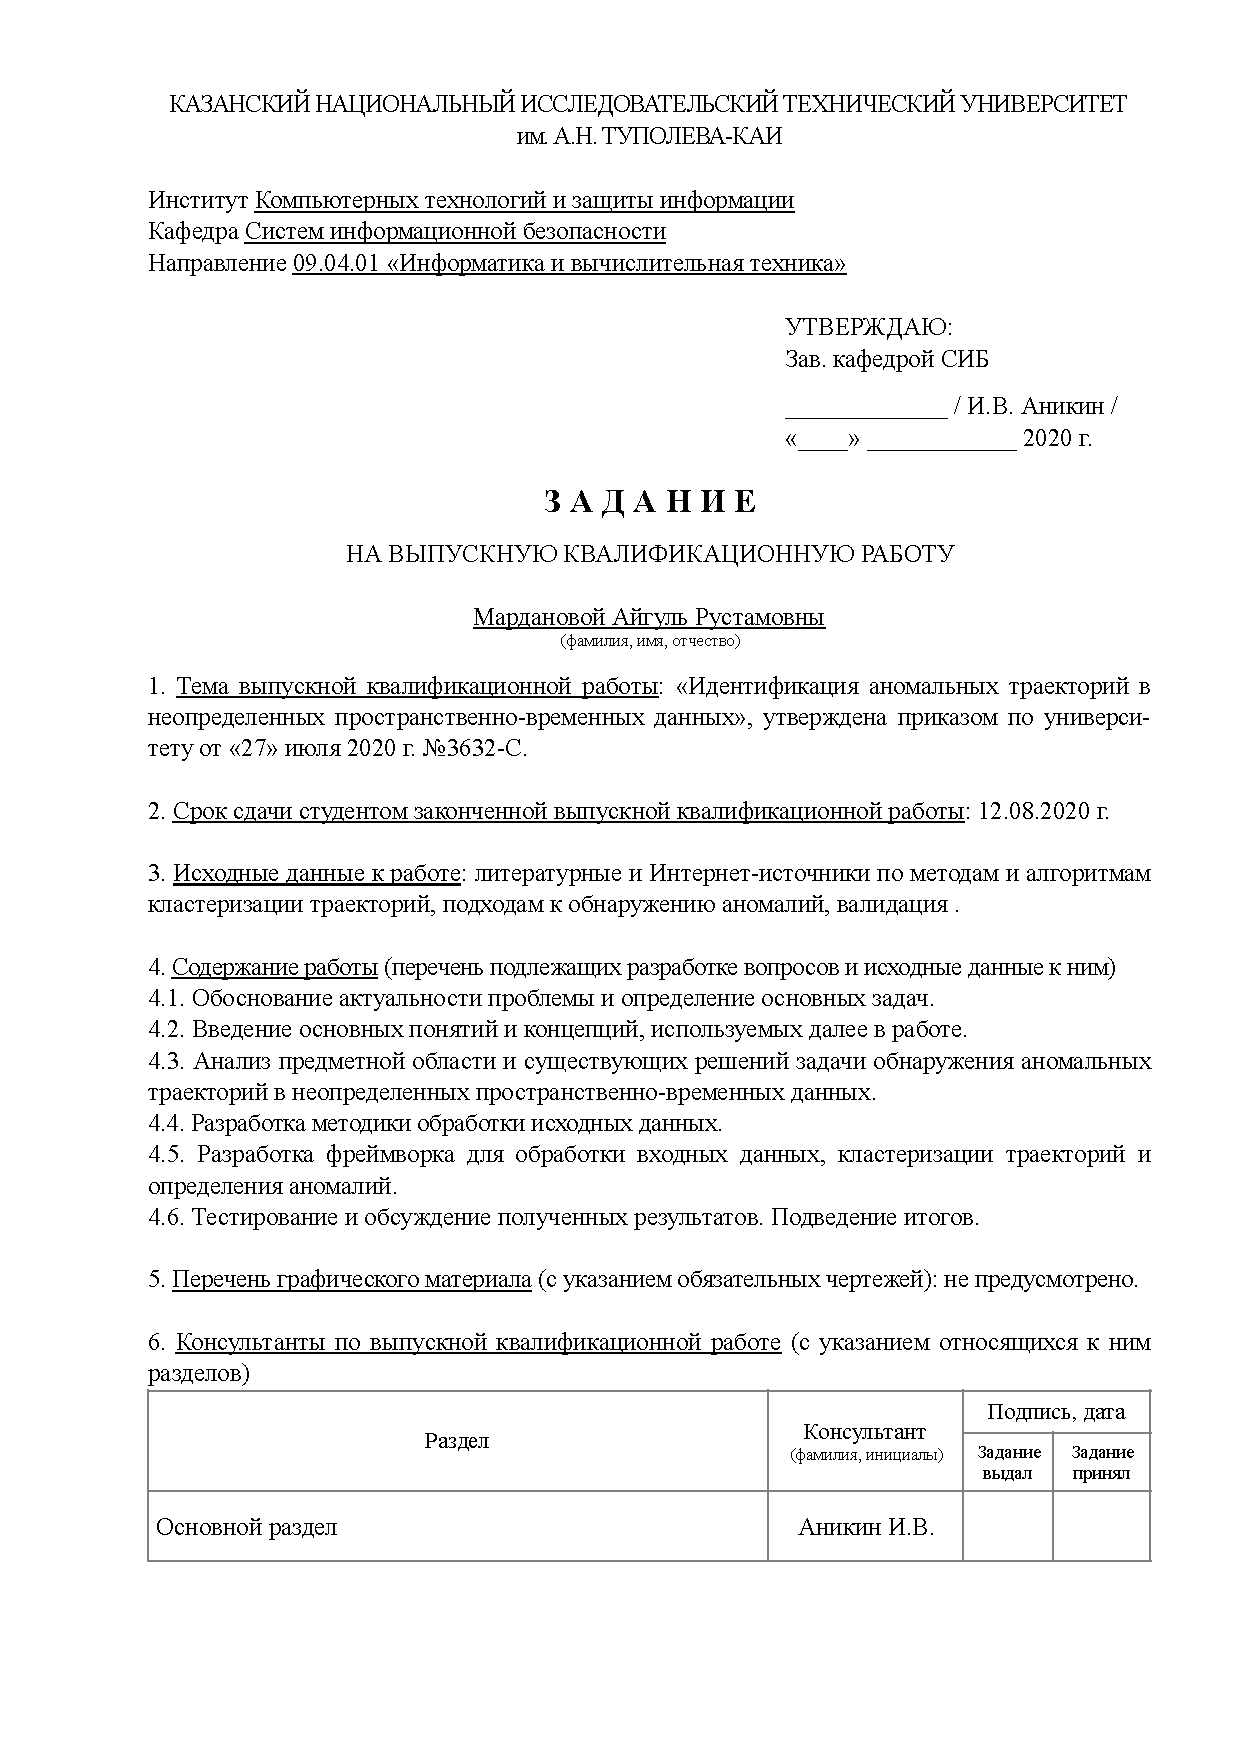
\includepdf[page={1,2}]{include/zadanie}

\clearpage

%%%%%%%%%CONTENT%%%%%%%%%
\pagenumbering{arabic}
%\tableofcontents

\section*{Список сокращений}
\addcontentsline{toc}{chapter}{Список сокращений}
\label{ch:Список сокращений}
\markboth{Список сокращений}{}

\begin{tabular}{lll}
	\\
	\textbf{ГИС}        & & {Географические Информационные Системы} \\[0.5ex]
	\textbf{ИТС}        & & {Интеллектуальные Транспортные Системы} \\[0.5ex]
	\textbf{ТС}         & & {Транспортное Средство} \\[0.5ex]
	\textbf{ПДД}        & & {Правила Дорожного Движения} \\[0.5ex]
	\textbf{ДТП}        & & {Дорожно-Транспортное Происшествие} \\[0.5ex]
	\textbf{GPS}		& & {Global Positioning System} \\[0.5ex]
	\textbf{ID}			& & {Identificator} \\[0.5ex]
	\textbf{SVM}		& & {Support Vector Machine} \\[0.5ex]
	\textbf{DBSCAN}		& & {Density-Based Spatial Clustering of Applications with Noise} \\[0.5ex]
	\textbf{DTW}        & & {Dynamic Time Warping} \\[0.5ex]
	\textbf{LCSS}       & & {Longest Common SubSequence} \\[0.5ex]
	\textbf{HMM}       	& & {Hidden Markov Model} \\[0.5ex]
	\textbf{DI}			& & {Dunn's Index} \\[0.5ex]
	\textbf{AWT}		& & {Abstract Window Toolkit} \\[0.5ex]
	\textbf{ИПП}        & & {Интерфейс Прикладного Программирования} \\[0.5ex]
	\textbf{API}		& & {Application Programming Interface} \\[0.5ex]	
	\textbf{ГПИ}        & & {Графический Пользовательский Интерфейс} \\[0.5ex]
	\textbf{GUI}		& & {Graphical User Interface} \\[0.5ex]
	\textbf{FARS}       & & {Fatality Analysis Reporting System} \\[0.5ex]
	\textbf{SSE}        & & {Sum of Squares due to Error} \\[0.5ex]
	\textbf{TSS}        & & {Total Sum of Squares} \\[0.5ex]
	
	
\end{tabular}
		% Перечень сокращений
\section*{Перечень обозначений}
\addcontentsline{toc}{chapter}{Перечень обозначений}
\label{ch:Перечень обозначений}
\markboth{Перечень обозначений}{}

\begin{tabular}{lll}
	\\
	$\bm{\tau}$, $\bm{T}$       	& & {Траектория} \\[0.5ex]
	$\bm{TP}$        				& & {Точка Траектории} \\[0.5ex]
	$\bm{t}$						& & {Временной параметр} \\[0.5ex]
	$\bm{x}$						& & {Координата X} \\[0.5ex]
	$\bm{y}$						& & {Координата Y} \\[0.5ex]
	$\bm{\upsilon_{avg}}$			& & {Средняя скорость траектории} \\[0.5ex]
	$\bm{d_{ij}}$					& & {Евклидово расстояние между траекториями $T_i$, $T_j$} \\[0.5ex]
	$\bm{dist(a_i^k, b_j^k)}$		& & {Евклидово расстояние между точками $a_i^k$, $b_j^k$} \\[0.5ex]
	$\bm{R^2}$						& & {Коэффициент детерминации R-квадрат} \\[0.5ex]
	
\end{tabular}
			% Перечень обозначений
\chapter*{АННОТАЦИЯ}

Работа состоит из 93 страниц, содержит \TotalValue{totalfigures} рисунок, \TotalValue{totaltables} таблиц, 48 источников, 4 приложений.

В данной работе решается задача анализа пространственно-временных данных о траекториях транспортных средств с целью выявления частых траекторий движения и обнаружения аномальных траекторий с учетом неопределенности. Одной из основных пробелом, исследованных в работе, является неопределенность исходных пространственно-временных данных, возникающая в результате использования данных с камер видеонаблюдения и ведущая к потере качества результатов кластеризации траекторий, дальнейшей их классификации и обнаружения аномалий. 

В ходе выполнения работы были рассмотрены основные существующие подходы к анализу траекторий, полученных с камер видеонаблюдения, и, в частности, к решению задачи обнаружения аномалий, проанализированы причины и особенности неопределенности исходных данных. Был предложен подход для решения поставленной задачи, исследована возможность повышения точности результатов и разработан метод для минимизации влияния неопределенности данных, заключающийся в том, что необходимо учитывать расположение движущегося транспортного средства по отношению к камере. Для реализации предложенного подхода, проведения оценочных тестов и визуализации результатов была разработна платформа.

\bigbreak
Ключевые слова: пространственно-временные данные, кластеризация траекторий, обнаружение аномальных траекторий, неопределенность пространственно-временных данных.		% Аннотация
\chapter*{ABSTRACT}

The work consists of 93 pages, contains \TotalValue{totalfigures} figures, \TotalValue{totaltables} tables, 48 sources, 4 appendices.

Nowadays spatiotemporal data analytics plays an important role, and this work is intended to solve the task of analyzing spatiotemporal data, representing vehicle trajectories, to perform frequent trajectory patterns mining and detection of trajectory anomalies with the consideration of uncertainty of data. The uncertainty, arising from the use of data from CCTV cameras, can lead to a loss in the quality of trajectory clustering results, their further classification and anomaly detection.

In the course of this work, the main existing approaches to analyze trajectories obtained from CCTV cameras, and, in particular, to solve the problem of detecting anomalies were considered, the reasons and features of the uncertainty of the initial data were inspected. As results, an approach to solve the problem was proposed, the possibility of improving the accuracy of the results was investigated, and a method was developed to minimize the effect of data uncertainty, which consists in the fact that it is necessary to take into account the location of a moving vehicle in relation to the camera. To implement the proposed approach, conduct assessment tests and visualize the results, a platform was developed.

\bigbreak
Key words: spatiotemporal trajectory data, spatiotemporal data uncertainty, trajectories clustering, trajectory anomalies detection.		% Абстракт на англ
\chapter{ВВЕДЕНИЕ}
\label{ch:ВВЕДЕНИЕ}

В наши дни обработка и анализ пространственно-временных данных приобретает все большую популярность и находит все большее применение в приложениях, основанных на использовании Географических Информационных Систем (ГИС). Последние исследования в области ГИС и, в частности, технологий и инфраструктуры для ГИС способствовали развитию интеллектуальных городов. И Интеллектуальные Транспортные Системы (ИТС), подразумевающие анализ городского транспортного движения, являются одной из самых перспективных областей \cite{article:2_survey_urban}.

Интеллектуальное слежение в умных городах получило большое развитие за последнее десятилетие \cite{article: 9_trb_vc_aev_sc}. В последнее время растущее число дорог и общественных мест оснащаются видеокамерами для мониторинга, увеличивается количество общедоступных видеоданных для анализа \cite{article:4_detect_eatp}. Задача автоматического анализа данных, собранных в ходе видеонаблюдения за дорожным движением, привлекает все большее внимание научного сообщества \cite{inproceedings:21_ad_dbscan_tvs}.

В настоящее время существует множество задач и применений анализа городского транспортного движения, однако, согласно \cite{article:9_trb_vc_aev_sc}, отслеживание поведения транспортных средств (ТС) с помощью обработки видео-изображений является одним из самых многообещающих подходов. Одним из основных исследовательских подходов в области анализа городского трафика, предполагающих работу с данными с камер видеонаблюдения, является извлечение из пространственно-временных данных паттернов частых траекторий движения. Извлеченные траектории могут впоследствии быть применены для автоматического визуального наблюдения, регулирования транспортного движения, обнаружения подозрительных активностей и др. \cite{article:5_survey_tbsa}\cite{article:over_tod}. 

Еще одной важной подкатегорией в области анализа трнаспортного трафика является обнаружение аномалий в потоке данных \cite{article:9_trb_vc_aev_sc}. Данная задача является очень актуальной и находит применение во многих приложениях для умных городов. Аномалия традиционно характеризуется как событие, экземпляр данных, который значительно отличается от большинства экземпляров в наборе данных и отклоняется от нормы \cite{article:1_survey_stdm}. В сфере видеонаблюдения за ТС аномальной деятельностью обычно называют события, которые нарушают общие закономерности, как правило, правила дорожного движения (ПДД) \cite{inproceedings:21_ad_dbscan_tvs}. Такие необычные паттерны движения ТС, которые не соответствуют ожидаемому поведению, несут важную информацию, поскольку могут свидетельствовать об аномальных транспортных потоках в сети автомобильных дорог \cite{article:9_trb_vc_aev_sc}. Например, случаи дорожно-транспортного происшествия (ДТП) или затора в транспортном движении ведут к резкому изменению транспортных потоков. Это в свою очередь провоцирует появление траекторий движения, отклоняющихся от нормальных паттернов движения. Следовательно, распознавание аномалий может быть полезно для своевременного обнаружения случаев ДТП и предпринятия должных мер. Однако, в наш век информационного перенасыщения, когда огромные массивы данных доступны для обработки и анализа, ручная и обработка становится невыполнимой задачей, неавтоматизированные решения становятся невозможными и неподходящими из-за высокой степени сложности и времязатратности. Поэтому исследования научных сообществ направлены на разработку автоматических и полуавтоматических интеллектуальных методов для решения этих задач с максимально возможной минимизацией необходимости вовлечения человека-оператора \cite{article:19_gbta_ubd_is}.

Как отмечается в последних исследованиях в области анализа транспортного трафика, во многих приложениях, включая ИТС, чрезвычайно важно учитывать неопределенность данных. Причины неопределенности данных разнообразны. Например, неопределенность данных может быть в результате неточности измерений или неточности наблюдений. В случае получения данных о траектории с камер видеонаблюдения неопределенность данных может быть вызвана ограничениями используемых устройств или потерянным местоположением \cite{inproceedings:14_mpfstsp_gp_ud}.

\section{Постановка задачи}

Как было отмечено выше, в наши дни анализ пространственно-временных данных играет важную роль в ежедневных процессах, в повседневной жизни, и процесс извлечения полезной информации из пространственно-временных данных является одной из ключевых задач и проблем при анализе данных трафика. Поскольку пространственно-временные данные о траекториях ТС являются многомерными и пространственно-временны характеристики траектории зависимы между собой, традиционные подходы к анализу данных, предлагаемые для статических, единичных и независимых данных, становятся неэффективны и неуместны \cite{article:8_review_mot_cl_alg}. 

Основной целью работы в этом тезисе является разработка подхода к обработке неопределенных пространственно-временных данных о траекториях для решения задач определения частых траекторий и обнаружения аномалий, а также проведение сравнительного анализа предложенного решения. В качестве основы для проведения оценочных и контрольных тестов, направленных на проверку точности и эффективности предложенного подхода, будет разработан фреймворк (платформа) для извлечения часто встречающихся траекторий и обнаружения наомальных траекторий в трехмерных пространственно-временных данных траекторий, полученных с камер видеонаблюдения. Видео с камер наблюдения будет обрабатываться во внешней системе слежения, которая извлекает траектории ТС и преобразует их в векторы, состоящие из точек слежения (точек траектории). Внедренный метод должен быть оценен с точки зрения точности и производительности, а также способности улучшить, повысить точность результатов в контексте таких особенностей входных данных, как неопределенность.

Для решения вышеупомянутых проблем следующие задачи должны быть выполнены:

\begin{itemize}
	\item Провести анализ предметной области и существующих подходов и выбрать методы для решения задач определения частых траекторий движения и обнаружения аномалий;
	\item Исследовать возможность улучшения существующего метода и предложить метод для повышения точности результатов для выбранного метода в контексте использования данных с камер видеонаблюдения;
	\item Реализовать фреймворк с использованием выбранных алгоритмов для тестирования предложенного похода и проведения сравнительного анализа полученных результатов;
	\item Провести тестирование эффективности и точности рализованного подхода.
\end{itemize}

Эта работа будет сфокусирована на следующих типах аномальных траекторий:

\begin{itemize}
	\item Аномальные траектории с аномальной пространственной информацией. Эта категория покрывает траектории с аномальным пространственным поведением, такие как запрещенные на перекрестках развороты на 180$^{\circ}$, пересечение двойной сплошной линии, движение в обратном направлении.
	\item Аномальные траектории с аномальной пространственно-временной информацией. Этот тип аномалий относится к случаям, когда пространственная информация сама по себе может быть расценена как нормальная, но вместе с информацией о времени представляет собой аномальное поведение, например: движение с чрезвычайно высокой или низкой скоростью, неожиданные аварийные остановки.
\end{itemize}

\section{Структура работы}

Работа структурирована следующим образом. Весь отчет состоит из 7 частей. Первая часть представляет собой введение, где описана актуальность работы, обозначены цели и задачи, структура отчета. Во 2 главе вводятся основные понятия и необходимая терминология, используемая далее в работе. Глава 3 посвящена результатам анализа литературы в предметной области и обсуждению современного состояния поставленной проблемы. В главе 4 приведено подробное описание предлагаемого подхода к решению поставленной задачи на концептуальном уровне, с алгоритмическим описанием используемых методов и архитектурных особенностей. Глава 5 описывает детали реализации фреймворка, формат структуры входных данных и процесс обработки входных данных. В главе 6 представлена подробная информация о подготовке экспериментов и приведены результаты проведения экспериментов, направленных на тестирование точности и эффективности использованных методов. Глава 7 представляет собой заключение и содержит краткое изложение полученных результатов и обсуждение дальнейших перспектив развития. В Приложении приведен исходный код для ключевых алгоритмов из реализованного фреймворка, подкрепленных описанием и комментариями, представленными в главе 5. 	% Введение
\chapter{ОСНОВНЫЕ ПОНЯТИЯ}
\label{ch:ОСНОВНЫЕ ПОНЯТИЯ}

Эта глава предназначена для предоставления справочной информации, введения полезных определений и основных концепций подходов, используемых в следующих главах. В этой главе будут рассмотрены источники входных данных и связанные с ними проблемы.

\section{Источники входных данных}

Задачи определения частых траекторий и обнаружения аномалий могут быть реализованы применимо к различным источникам данных, например: устройства GPS (Global Positioning System, глобальная система позиционирования) и сенсорным сетям, когда данные о траектории собираются датчиками на движущихся объектах, которые периодически передают информацию о местоположении движущегося объекта во времени, или камеры видеонаблюдения. Данная работа будет сфокусирована на работе с последним типом источников входных данных.

Видеоданные с камер слежения являются необработанными данными и не используются непосредственно в качестве входных данных для разрабатываемой системы. Обработка необработанного видео выполняется в автономной системе слежения. Система слежения берет исходное видео с камер видеонаблюдения и обрабатывает его, выполняя обнаружение объектов и преобразовывая траекторию в ряд точек слежения на изображениях. Точки слежения, содержащие такую информацию, как идентификатор (ID) ТС, метку времени, пространственные координаты, используются в качестве входных данных.

\section{Определение траектории}

Траектории могут быть представлены как многомерные последовательности, содержащие упорядоченный во временном отношении список местоположений вместе с любой дополнительной информацией \cite{article:1_survey_stdm}. Таким образом, поскольку траектория, обозначенная как $\tau$ или $T$, представляет собой последовательные местоположения движущегося целевого объекта во времени, в случае получения данных наблюдения с одной камеры ее можно определить как:

\begin{equation}
	\tau = T = {(x_1, y_1, t_1), (x_2, y_2, t_2), \ldots, (x_n, y_n, t_n)}\\[3pt]
\end{equation}

где пары $(x_i,y_i)$ обозначают положение целевого объекта на изображении в момент времени $t_i$ \cite{article:5_survey_tbsa}. В соответствии с этим траектории могут быть представлены в виде последовательности трехмерных точек, где 2D-объект предназначен для геометрических координат, а в третьем измерении хранится время \cite{article:25_dhr_mvt_eesd}.

Как правило, данные о траекториях являются сырыми, необработанными и содержат только минимальную информацию, такую как положение в пространстве и время, а также ID объекта отслеживания. Указанная информация может быть легко дополнена такой подробной информацией, как скорость, ускорение и направление, поскольку они могут быть извлечены из исходных данных о траектории \cite{article:12_dssto_mot}.

\subsection{Определение аномальной траектории}

Двадцатичетырехчасовые записывающие камеры видеонаблюдения производят огромные объемы данных о движущихся объектах, и это увеличивает вероятность того, что наряду с объектами, имеющими нормальное поведение, некоторые из движущихся объектов будут демонстрировать ненормальное поведение. Такое исключительное поведение можно также назвать исключением, аномалией, отклонением (от нормы) \cite{article:11_eod_hdd}\cite{article:15_survey_ad}. Несмотря на то что не существует стандартизированного определения понятия аномалии, в статистике можно найти следующую расшифровку данного понятия \cite{article:13_pdoos}:

\begin{quote}
	``An outlying observation, or outlier, is one that appears to deviate markedly from other members of the sample in which it occurs''.
\end{quote}

Траекторные аномалии (или аномальные траектории) могут быть описаны как паттерны потока транспортного трафика, значительно отклоняющиеся от некоторого нормального шаблона поведения или, другими словами, несовместимые с остальными моделями поведения трафика. Предполагается, что аномальные траектории имеют большую локальную или глобальную разницу с большинством траекторий согласно выбранной метрике подобия \cite{article:over_tod}.

Процесс обнаружения аномалий направлен на выявление необычных паттернов, которые кардинально отличаются от большинства экземпляров в исходных данных, для дальнейшей их обработки соответствующим образом \cite{article:11_eod_hdd}. Также необходимо отметить, что отношение аномальных паттернов траекторий к нормальным моделям активности должно быть относительно небольшим, чтобы можно было отличить аномалии от доминирующих нормальных паттернов.

\subsection{Классификация аномальных траекторий}

Согласно литературе, аномальные траектории могут быть классифицированы следующим образом \cite{article:15_survey_ad}\cite{article:6_survey_anom_det_rtuvs}\cite{article:comp_analys_odt}:
\begin{itemize}
	\setlength\itemsep{-0.5em}
	\item \textit{Точечная аномалия, Point anomaly} -- представляет собой наипростейший тип аномалий. Соответствует отдельному экземпляру данных, который расценивается как аномальный по отношению к остальному массиву данных, поскольку он значительно отличается от всех других экземпляров в наборе данных. Например, неподвижная машина на оживленной дороге.
	\item \textit{Контекстная аномалия, Contextual anomaly} -- экземпляр данных, который является аномальным в определенном контексте, но может быть нормальным в другом случае. Контекстная аномалия может также быть представлена как точечная в своем локальном окружении аномалия. Контекстуальные аномалии также называются условными аномалиями и представляют собой наиболее распространенную группу категорий, применимых к пространственно-временным данным. Например, траектории могут быть классифицированы на основе пространственных данных (координат) в пределах времени. Примерами контекстных аномалий могут быть траектории движения ТС с гораздо более высокой скоростью по сравнению с другими в том же транспортном потоке или движения ТС в противоположном направлении.
	\item \textit{Собирательные аномалии, Collective anomalies} -- множество экземпляров данных, которые в совокупности как группа представляют собой аномалию по отношению к остальной части данных, в то время как каждый экземпляр данных в отдельности не обязательно является аномальным. Данное определение может быть упрощено до следующей формы: набор соседних точечных аномалий или контекстных аномалий. Коллективные аномалии могут быть применены только к наборам данных, в которых существует зависимость между экземплярами данных
\end{itemize}

Другим способом систематизации аномальных траекторий может быть разделение их на следующие категории в соответствии со свойствами, которые использовались для выполнения классификации:

\begin{itemize}
	\setlength\itemsep{-0.5em}
	\item \textit{Пространственные аномальные траектории, Spatial trajectory anomaly} -- классификация учитывает только пространственную информацию о траекториях движущихся объектов, например координаты местоположения. Примерами пространственных аномалий могут быть незаконные развороты, пересечение двойной сплошной линии или движение в противоположном направлении.
	\item \textit{Временные аномальные траектории, Temporal trajectory anomaly} -- аномалии, обнаруженные путем анализа только временных характеристик траекторий, таких как продолжительность, время перемещения. Например, траектория со значительно большей продолжительностью или траектория, появляющаяся в аномальное время.
	\item \textit{Пространственно-временные аномальные траектории, Spatiotemporal trajectory anomaly} -- могут быть обнаружены путем анализа пространственной и временной информации в совокупности. Примерами пространственно-временных аномалий могут быть траектории ТС, движущихся со значительно высокой скоростью по сравнению с большинством траекторий. Также такие аномалии могут быть обнаружены в случае транспортных систем с реверсивным движением. Так как для таких полос движения разрешено изменение направления согласно некоторому известному или изученному графику, классификатор может анализировать направление траектории вместе с информацией о времени.
\end{itemize}

В соответствии со второй классификацией эта работа будет сфокусирована на определении аномальных траектории первого и третьего типов (пространственных и пространственно-временных аномальных траекторий).

\section{Основные сложности}

Поскольку пространственно-временные данные отличаются от других типов данных во многих аспектах, сложности связаны с используемым этого типа данных. Уникальным качеством пространственно-временных данных является то, что экземпляры данных не являются независимыми и одинаково распределенными, как это обычно предполагается во многих существующих подходах для интеллектуального анализа данных. Напротив, экземпляры пространственно-временных данных, связанные с результатами наблюдения, проведенными в близлежащих точках и близкое время, структурно коррелируют друг с другом в контексте пространства и времени, и важно учитывать наличие зависимостей между значениями в этих измерениях. Следовательно, многие из существующих подходов для интеллектуального анализа данных не применимы к пространственно-временным данным, поскольку игнорирование вышеупомянутых характеристик может привести к низкой точности результатов. Это ведет к необходимости изучения и использования различных методов обработки таких данных для сохранения всех связей между информационными доменами \cite{article:1_survey_stdm}.

\subsubsection{Неопределенность данных}

Также следует отметить, что выбранный тип источника данных приводит к трудностям при обработке. Поскольку данные о траектории собираются с видеокамер, первая проблема заключается в неопределенности местоположения в результате ограничений точности измерений используемых камер, разрешения и качества полученных изображений, дрожания кадра \cite{article:4_detect_eatp}. Кроме того, камеры слежения размещаются в определенных фиксированных местах на перекрестках, из-за чего одной из особенностей используемых данных являются положение движущегося объекта и перспектива, которые могут вызвать проблемы при работе с входными видеоданными \cite{article:6_survey_anom_det_rtuvs}. Угол обзора камеры относительно земной горизонтальной поверхности и расстояние между отслеживаемым объектом и камерой могут влиять на качество обработки, понижая точность обнаружения и отслеживания объектов: чем меньше угол, тем существеннее проблема определения центра объекта \cite{article:4_detect_eatp}\cite{article:9_trb_vc_aev_sc}. Отслеживаемые объекты могут въезжать и выезжать в поле / из поля зрения камеры, но при этом оставаться отслеживаемыми, посколько они частично видны. Это может привести к изменению траектории на границах поля зрения камеры: смещение траекторий ТС в зависимости от расположения объекта относительно камеры \cite{article:4_detect_eatp}. Качество извлечения и последующего анализа траекторий также зависит от входных данных о траекториях, включая такие критерии, как качество используемых камер, качество системы слежения, которая преобразует видеоданные в список траекторий, состоящий из точек слежения.

Более того, в текущей дипломной работе входные данные содержат траектории, извлеченные из видеокамер без фильтрации и предварительного анализа, поэтому:

\begin{enumerate}
	\setlength\itemsep{-0.5em}
	\item входные данные содержат экземпляры и нормальных, и аномальных траекторий;
	\item входные данные содержат траектории без указания меток классов.
\end{enumerate}

Вышеупомянутые ограничения ведут к необходимости использовать неконтролируемые безнадзорные методы для автоматического извлечения паттернов нормальных и аномальных траекторий движения из непомеченных, неклассифицированных данных \cite{article:27_vna_cad_td}.
 				% Basic Knowledge
\chapter{АНАЛИЗ ПРЕДМЕТНОЙ ОБЛАСТИ}
\label{ch:АНАЛИЗ ПРЕДМЕТНОЙ ОБЛАСТИ}

This chapter presents state of the art analysis of existing approaches and discusses advantages and disadvantages of existing approaches. Each section is concluded with a summary, in which the chosen approach is specified and a short argumentation is given.

\section{Методы обнаружения аномалий}
According to \cite{article:15_survey_ad}, the task of outliers detection, which is a main objective task of this work, has been an object of interest and studies of research community originating from $19\up{th}$ Century. Nowadays a huge variety of different techniques for solving the task of detecting outliers and abnormalities in video traffic data are presented, and these approaches can be classified in various ways.

For example, data mining techniques in general and anomaly detection techniques as well as clustering approaches, which are one of the ways to solve the task of outliers identification, particularly can be classified as supervised, semi-supervised and unsupervised on the grounds of the manner of labeling the input data] \cite{article:15_survey_ad}\cite{article:comp_analys_odt}:
\begin{enumerate}
	\item \textit{Supervised}. Input data used for training contains labels for both normal and anomalous instances. As a result the algorithm can build models for both normal and abnormal classes;
	\item \textit{Semi-Supervised \cite{article:15_survey_ad}} or \textit{Weakly-Supervised \cite{article:5_survey_tbsa}}. Input training data set contains class labels only for normal data instances. Such techniques are more widely used than supervised approaches, since anomalous data instances are usually not predictable and random and it is difficult to provide examples to cover all possible anomalous events;
	\item \textit{Unsupervised}. Does not require input data to be labeled neither for normal nor anomalous data. Such algorithms are based on the expectation that normal data instances are significantly more frequent than anomalous ones in the test data set and therefore are not applicable when this assumption is disrupted.
\end{enumerate}

Alternatively, according to surveys done by Chandola in \cite{article:15_survey_ad}, Kumaran in \cite{article:6_survey_anom_det_rtuvs} and Malik in \cite{article:comp_analys_odt}, anomaly detection techniques can be classification based, nearest-neighbor based, clustering based, statistical and etc. The following offers the short overview of mentioned groups.

\subsubsection{Основанные на кластеризации}
The main concept of these methods lies in using a classifier which firstly learns to distinguish inliers and outliers and then classifies each input instance \cite{inproceedings:18_ardod_lstd}. Such techniques consist of training and testing phases. Training, or learning, phase supposes learning a classifier model from a training data set, containing labeled data instances. The learned classifier is then used to classify an input trajectory as normal or anomalous by assigning a class label in a testing phase.

Depending on how testing data instances are labeled, all classification based anomaly detection techniques can be one-class or multi-class. The first type assumes that all training data instances are normal and are labeled as one class. During training phase model learns a discriminative boundary around normal instances, and a trajectory, which is not aligned with the learned normal class description, is considered as an anomalous. Single-class Support Vector Machines (SVMs) is the most commonly used classification based approach, which is applicable to the task of anomalous trajectory detection, as it was proposed by Piciarelli \textit{et al.} \cite{inproceedings:16_va_tad_svm}\cite{article:17_tbaed}. However, this approach requires trajectory vectors to be the same length. Since raw trajectory data is usually contains different amount of trajectory points due to different speed of moving objects, it is necessary to preprocess raw trajectories to normalize them to vectors of the same length \cite{article:17_tbaed}. Moreover, SVMs become highly time and memory consuming while working with huge amounts of multi-dimensional data \cite{article:22_survey_dscc}.

The latter category supposes learning multiple classes during training step and then using a classifier to review the input trajectory for compliance with each learned class. In literature different descriptions of training phase and training data labels are given. According to \cite{article:15_survey_ad}, training data contains only normal data instances with corresponding normal class labels, and during training phase model learns multiple discriminative boundaries around each class of normal instances. A trajectory, which is aligned with none of the learned normal class descriptions, is considered as an anomalous. In other words, an anomalous trajectory will not be accepted by neither of the classifiers. In \cite{article:6_survey_anom_det_rtuvs} it is assumed that model is learned using training data containing labels for normal and anomalous classes. Therefore, a classifier can classify an input trajectory as belonging to a normal or anomalous class.

The advantage of two-phased classification based algorithms is a fast testing phase due to precomputed classifier model used to classify each input instance. Also such algorithms can perform well in cases when anomalous data instances form a class or cluster \cite{inproceedings:18_ardod_lstd}. However, the training step requires accurately labeled training data, which is often not available. 

\subsubsection{Основанные на методе ближайших соседей \cite{article:15_survey_ad} или Основанные на близости / плотности распределения \cite{article:6_survey_anom_det_rtuvs}\cite{inproceedings:18_ardod_lstd}}
Proximity based approaches decide whether a data instance is normal or anomalous based on how close or far is it located with respect to neighbors \cite{article:6_survey_anom_det_rtuvs}. Nearest-neighbor and density based approaches are based on the assumption, that «normal data instances have dense neighborhood, while anomalous data instances occur far from their closest neighbors» \cite{article:15_survey_ad}.

In order to be able to compare the surrounding density for an instance under consideration with the density around its local neighbors, a distance (dissimilarity) or similarity measure between two data instances needs to be specified \cite{inproceedings:18_ardod_lstd}. By virtue of an anomaly score calculation method, techniques can be grouped into two categories: 1) the anomaly score is calculated as a distance of a data instance to its $k^th$ nearest neighbor and 2) to compute the anomaly score the relative density of each data instance is being computed \cite{article:15_survey_ad}.

These approaches has several disadvantages. First of all, in comparison with classification based anomalies detection techniques, the computational complexity of the testing phase is considerably higher, since nearest neighbors are computed by computing the distance for each test data instance with all instances from either testing and training data. In case of multi-dimensional trajectory data, the task of distance computation becomes even more complicated. Moreover, the accuracy of labeling decreases when the main assumption is violated: when normal instances have sparse neighborhood or anomalous instances have dense \cite{article:15_survey_ad}.

\subsubsection{Основанные на кластеризации}
Clustering is an efficient approach aimed to group data instances into different classes, called clusters, based on their similarity in such a way, that objects in one cluster are similar to each other and dissimilar to objects in other clusters \cite{article:8_review_mot_cl_alg}\cite{article:22_survey_dscc}. ST clustering supposes grouping objects on the ground of their spatial and temporal similarity. To compare data instances before grouping them into clusters, similarity or distance between them needs to be measured.

There are three types of clustering based anomalies detection techniques with following assumptions: 1) normal data instances are associated with a cluster, while anomalous data instances are not associated with any cluster, 2) normal data instances are close to the cluster center, while abnormal instances lie far away from the closest cluster center and 3) normal data instances lie in large and dense clusters, while anomalies are associated with sparse clusters or clusters with a small cardinality \cite{article:15_survey_ad}\cite{article:6_survey_anom_det_rtuvs}. Techniques of first type can be implemented using one of the clustering methods which do not require every data instance to belong to some cluster, for example DBSCAN \cite{inproceedings:20_dbscan}. Algorithms from second group consist of two phases: 1) data clustering and 2) calculating an anomaly score for each data instance. Techniques of the latter type require a threshold for cardinality size and/or density of a cluster to be defined to decide whether a cluster refers to normal or anomalous data.

The necessity to compute distance between trajectories in some of the clustering based approaches makes them similar to neighbor based approaches. As it is stated in \cite{article:15_survey_ad}, techniques are different in the way they process instances: in clustering based techniques each instance is evaluated with respect to the corresponding cluster, while in neighbor based techniques each instance is being inspected with respect to its proximate neighborhood. Consequently, the selection of distance computation method plays an important role and affects results and performance significantly.

On the other side, dividing all training data into groups makes clustering based algorithms similar to classification based algorithms. Though in classification based approaches class is assigned based on given labels, while in clustering based approaches classification is not given in advance \cite{inproceedings:18_ardod_lstd}.

One of the main advantages of clustering based techniques is the ability of majority of them to run in an unsupervised manner. For the case of TVS-based trajectory data acquisition the unsupervised learning methods are the most appropriate, because labeling hours of video data is a highly time-consuming task. Also, manual labeling of input data can lead to errors due to human operator intervention.

Moreover, clustering based techniques are adjustable to work with complex data types because of adaptability of clustering algorithms. However, at the same time they are computationally expensive and are used primarily for relatively low dimensional data, highly dependent on the used clustering algorithm and can not effectively deal with situations when anomalies form significant separate cluster groups \cite{article:15_survey_ad}.

\subsubsection{Методы с применением моделей  \cite{article:6_survey_anom_det_rtuvs}\cite{inproceedings:18_ardod_lstd} или Статистические \cite{article:15_survey_ad}}
The main concept of model based algorithms is that they represent the data as a set of parameters to create the model of a normal behavior. As an advantage, model based approaches do not ask the user to provide any input parameters, because all the parameter values can be derived from the data. Statistics based approaches can be considered as a subcategory of model based approaches, they are treated as one of the earliest algorithms and can be used as a basis by the various outlier detection techniques \cite{article:comp_analys_odt}. As it is stated in \cite{article:15_survey_ad}, the main idea of statistical approaches is that data instances occurring in high probability regions of a stochastic model assumed to be normal, while data instances from the low probability regions refer to anomalies. So, statistical approaches are based on using statistical stochastic model to fit to the given data and then applying a statistical inference test, also called discordance test, to decide if a data instance is normal or anomalous. It comes from the main concept that «based on results of applied statistical test, anomalies have low probability to be generated from the learned stochastic model» \cite{article:15_survey_ad}.

Statistical techniques in turn can be parametric or non-parametric \cite{article:comp_analys_odt}. In parametric approaches the normal data is supposed to fit the parametric distribution and probability density function with estimated from the given data parameters \cite{article:6_survey_anom_det_rtuvs}. One of the advantages of parametric techniques is that the data size does not affect the model: models grow only depending on a model complexity. However, the necessity to fit the data into some preselected distribution model complexifies and limits the application of such approaches: it is difficult to fit the data to one distribution. In this case it is possible to use a multiple-distribution model to match some clusters of the data with particular distributions \cite{inproceedings:18_ardod_lstd}. One of the most known examples of parametric methods is Regression Method \cite{article:comp_analys_odt}.

By contrast to this, non-parametric approaches are based on using non-parametric statistical models with structures, which are not defined in advance: the given data is used to determine the structure dynamically. Such approaches do not suppose making assumptions about the statistical distribution of the data \cite{article:comp_analys_odt}.

Since statistical approaches are based on fitting a statistical model, the choice of it significantly affects results, computational complexity and performance. Nevertheless, the main assumption of statistical approaches that the data comes from a particular distribution can not be always satisfied, specifically for the case of a multi-dimensional data \cite{article:15_survey_ad}.

\subsubsection{Выводы}
Based on the given description of different approaches and their advantages and disadvantages, it was decided to focus on clustering based anomalies detection approaches for several reasons: 
\begin{enumerate}[label=\arabic*)]
	\item they can work in an unsupervised mode without a human intervention and do not require the input data to contain labels,
	\item input data is allowed to contain anomalous trajectories,
	\item clustering method can be easily applied to such a multi-dimensional data as trajectories by defining a suitable similarity measure.
\end{enumerate}

That means that a clustering method and a similarity measure need to be specified.

\section{Классификация методов кластеризации}

Clustering is a highly researched form of data mining, and huge variety of clustering methods has already been proposed in literature \cite{article:8_review_mot_cl_alg}. State-of-the-art analysis of related research papers revealed that all traditional clustering approaches are usually categorized into five types: partitioning, hierarchical, density-based, model-based and grid-based methods \cite{article:5_survey_tbsa}\cite{article:8_review_mot_cl_alg}. Next paragraphs will briefly discuss each of the categories with highlighting main assumptions and concepts.

\subsubsection{Методы, основанные на разделении или декомпозиции}

Such methods are based on partitioning the trajectories data set randomly and then regrouping clusters by reassigning objects from one partition to another to minimize the objective function. They require the predefined parameter, usually denoted as $k$, which determines the amount of final clusters, or partitions, to be created. The main requirement is that number of partitions must be smaller than number of initial data points, since each partition forms a cluster, that means that it must be non-empty and contain at least one data instance, and each data instance must be included into exactly one cluster.

One of the most well-known examples of partitioning clustering algorithms is a $K$-Means algorithm, where firstly $k$ cluster centers are initialized randomly and then data points are iteratively reassigned to the closest clustering center based on the discrepancy to minimize the clustering error \cite{article:23_survey_ca}. The clustering error is defined as the sum of the squared Euclidean distances between each data set point and the corresponding cluster center \cite{article:24_glkkm_cl_fs}. The process is stopped when there are no more changes in clustering centers.

The disadvantages of the traditional K-Means clustering method are inability to form clusters of arbitrary form, dependence on initial random cluster centers initialization and high memory consumption \cite{article:8_review_mot_cl_alg}. Also finding an appropriate partitioning technique is a challenging task.

\subsubsection{Hierarchical methods}
In hierarchical based methods the given data set is decomposed into multiple levels to organize a hierarchical tree of clusters. The resulting hierarchical structure can be depicted as a tree \cite{article:23_survey_ca}.

There are two different ways of hierarchical decomposition: 1) the bottom-up (combining) and 2) the top-down (split, divisive) decomposition. They refer to agglomerative and divisive (split) clustering approaches respectively \cite{online:what_is_hier_clust}.

Agglomerative hierarchical clustering algorithms start by assigning each data instance to a distinct singleton-cluster, so the number of initial clusters is equal to the exact amount of data instances in input data, and then continue uniting clusters based on theirs similarity until all the initial clusters are merged into one single cluster or into predefined amount of clusters \cite{online:unders_hier_cl}. This is done by repeatedly executing following two steps: 1) identifying the two closest clusters and then 2) merging these two clusters \cite{online:what_is_hier_clust}. Proximity matrix is used to store similarity measurements between clusters and is being updated on each step by computing distances between the new cluster and the other clusters.

The divisive hierarchical clustering algorithms work in a reverse manner: initially all data instances belong to one cluster and then step by step clusters split into smaller clusters until all of them become singleton clusters or until satisfying some predefined end condition.

Hierarchical clustering is supposed to be simple, but it is necessary to choose between agglomerative and split methods. Divisive clustering is more expensive in computation, therefore, it is less common than agglomerative approaches. Irreversibility of both splitting or uniting processes in traditional hierarchical clustering algorithms is also a particularity of such algorithms \cite{article:8_review_mot_cl_alg}.

Since approach includes clusters joining, a significant task of agglomerative clustering algorithms is defining and computing the similarity or distance between clusters. This similarity can also be referred to as an inter-cluster or between-cluster distance. For the case of single-trajectory clusters the similarity between them is simplified and is equal to the similarity between respective trajectories. For multiple-trajectory clusters the similarity is computed according to a chosen linkage method. In literature following linkage methods are given as mostly common: single link, complete link, average link \cite{article:23_survey_ca}\cite{inproceedings:7_related_work}. The choice of the linkage method depends on the application domain \cite{online:what_is_hier_clust}. In the case of the single link distance between two clusters is defined as the minimum distance between two trajectories in these clusters, that means that the similarity between of two clusters is determined by two closest trajectories. The complete link linkage method implies taking the maximum distance between two trajectories in two clusters as an inter-cluster distance, so it is defined using the farthest distance of trajectory pairs. The average link supposes calculating averaged paired distance between all trajectory pairs in these two clusters.

A convenience of agglomerative hierarchical clustering approaches is that they do not require the number of resulting clusters to be predefined, so they are appropriate for clustering vehicle trajectories, because number of clusters of normal or anomalous trajectories is not known in advance. However, the most well-known disadvantage of hierarchical clustering algorithms is that they are not robust and can suffer from noise and anomalies. 

\subsubsection{Density-based methods}
In comparison with the partitioning and hierarchical clustering approaches, density-based methods objects inspect similarity based on the density of the data \cite{article:22_survey_dscc}. The area is being added to the nearest cluster, while density of the points in the area remains greater than the predefined threshold \cite{article:8_review_mot_cl_alg}. Clusters form dense regions of objects and they are separated by sparse regions with low density.

The main advantage of density-based clustering approaches is that they are able to form clusters of arbitrary forms, extend beyond spherical \cite{article:8_review_mot_cl_alg}. Also they are appropriate for clustering huge data sets of trajectories in an unsupervised manner and do not require the amount of clusters to be known in advance \cite{article:5_survey_tbsa}\cite{article:22_survey_dscc}. However, the results quality highly dependent on the amount of trajectories in training data set, available for analysis.

The most well-known and commonly used density-based algorithm is a DBSCAN, proposed by M. Ester \textit{et al.} in \cite{inproceedings:20_dbscan}. According to it, input data points are categorized as follows: core data, density-reachable data and outliers based on parameters $\varepsilon$, \textit{minPts} and the density threshold. Neighbor parameter $\varepsilon$ and \textit{minPts} specify the maximum remoteness and minimum amount of satisfying points while choosing the core points: at least \textit{minPts} points must be present within distance $\varepsilon$ from the core point, these points are marked as directly reachable from the chosen core point. Aforementioned parameters need to be predefined by the user, but it is difficult to determine them correctly. Each cluster must contain at least one core point. Points are denoted as anomalous if they are not reachable from any of the other points.

\subsubsection{Shrinkage-based or Grid-based methods}
The main idea of grid-based algorithms lies in applying a multi-resolution grid data structure: the data space is quantized into a finite number of cells (units) that form a multi-resolutional grid structure. Each cell stores summary information about data objects within its subspace \cite{article:22_survey_dscc}. Since clustering operations are performed on the created grid, and also important trajectories characteristics can be computed in each of the spatial grid cells, the quality of data compression influences the quality of results significantly \cite{article:1_survey_stdm}. Density of closely located dense cells can help to determine clusters. A trajectory can be considered as an anomalous if it differs from the expected trajectory in a number of covered grid cells \cite{article:22_survey_dscc}.

The main advantage of grid-based clustering algorithms is an improved performance: increased processing speed and processing time becomes independent on the size of the data set, only the number of cells in each dimension in the quantized space affects the processing time \cite{article:8_review_mot_cl_alg}.

\subsubsection{Model-based methods}
In comparison with the above methods, which analyze distance among data objects, in model-based approaches data is supposed to be generated by a mixture of probability distributions, where each component of mixture represents a cluster. So a mathematical model is assigned to each cluster, and then method attempts to find the best fitting data for the chosen model. In this way such methods seek to increase the adaptability between given data and some statistical models \cite{article:8_review_mot_cl_alg}\cite{article:22_survey_dscc}. The idea of model-based algorithms is that in order to locate clusters they describe the spatial distribution of the input data points by building density functions. The model-based approaches are typically used in feature-specific clustering and depend on the selected features and model \cite{article:5_survey_tbsa}.

It is emphasized, that model-based approaches show good performance while working with complex data types. This category usually includes statistical and neural network methods \cite{article:8_review_mot_cl_alg}.

\subsubsection{Graph-based methods \cite{article:1_survey_stdm}}
Another category of clustering methods in application to vehicle trajectories data. Liu \textit{et al.} in \cite{inproceedings:26_dstci_tds} presented a graph-based approach to solve the problem of detection of outliers in traffic data streams. A graph structure was used to store the traffic: nodes represent regions while edge weights depict the traffic flow. Edge anomalies in the graph denote the traffic abnormalities, and causal outlier tree can then be used to further analyze these outliers to find causal interactions.

\bigbreak
Another higher-level classification of clustering methods can consist of only two sub-classes on the ground of properties of generated clusters: hierarchical and partitioning approaches \cite{article:23_survey_ca}. Hierarchical algorithms group objects into clusters from singleton cluster to cluster containing all data instances or in a reverse direction. While partitioning clustering algorithms divide given data set into a predefined number of clusters in a single-layer structure.

In order to perform clustering, the similarity between two trajectories needs to be defined. Different existing distance measures will be reviewed in following paragraphs.

\subsubsection{Выводы}

Based on the given description of clustering approaches, their limitations, advantages and disadvantages, it was decided to focus on a hierarchical clustering approach, more specifically on an agglomerative hierarchical clustering, because it can deal with limitations of a given input data, that are: absence of input labels, unknown number of resulting clusters, presence of both normal and anomalous trajectories in input data.

\section{Метрики измерения близости и дальности}

As it was mentioned before, clustering based approaches require a similarity measure to be defined between two trajectories. Apart from that, distance and similarity measures are also used to compare a trajectory with a cluster or a pair of clusters between each other. A similarity measure highly dependent on the format of a trajectory. A trajectory data, represented as a multidimensional data, can contain quantitative or qualitative features, continuous or binary. In such a classification, distance measure functions are more appropriate to work with continuous features, while similarity measures – with qualitative features \cite{article:23_survey_ca}. Input trajectory-vectors in this work contain spatial information along with temporal, which can be termed as qualitative continuous data. That means that distance measure functions are more appropriate in this case. Moreover, distance and similarity functions can be classified as 1) working with raw representations of trajectories without any preprocessing steps and 2) working with preprocessed trajectories representations. Preprocessing can include unifying the length of trajectories or reducing the dimensionality of trajectory-vectors \cite{inproceedings:7_related_work}. 

Some of the most known and widely used traditional similarity measures are following: Euclidean Distance, Fréchet Distance, DTW, LCSS.

\subsubsection{Евклидово расстояние (Euclidean Distance)}

Euclidean distance between two trajectory vectors is calculated as a sum of squared differences of corresponding spatial coordinates \cite{article:27_vna_cad_td}:
\begin{equation}
	 d_{ij} = ||T_i - T_j||_E = \sqrt{\sum_{k=1}^{m}((t_{i_x}^k - t_{i_x}^k)^2 + (t_{i_y}^k - t_{j_y}^k)^2)},
\end{equation}
where both trajectories consist of \textit{m} tracking points and are represented by two-dimensional vectors $T_i = \{t_i^1, t_i^2, \ldots, t_i^m\}$ and $T_j = \{t_j^1, t_j^2, \ldots, t_j^m\}$. Tuples $(t_{i_x}^k, t_{i_y}^k)$ represent spatial coordinates for a \textit{k}-th tracking point of \textit{i}-th trajectory from a data set.

However, Euclidean distance works only with trajectories with equal number of tracking points. Since usually vehicles move with different speed and behavior, trajectory length is always different and that means that raw trajectories need to be preprocessed and reduced to the same size \cite{inproceedings:7_related_work}. Also, traditional Euclidean distance requires two-dimensional data, meaning that it is not able to process temporal information, and is dependent on the trajectory direction: the reversed direction can cause incorrect distance measurement, that in its turn leads to errors in clustering. Also, it fails while working with trajectories moving in a similar way but with different speeds and in the case of different sampling rates \cite{inproceedings:28_lcss_dsmt}.

\subsubsection{Расстояние Фреше (Fréchet Distance)}
Fréchet Distance is based on Euclidean distance. It considers the positional and sequential relationship of trajectory points while calculating the similarity. The main idea of this approach is computing Euclidean distance for each pair of points from two trajectories and then designating the maximum Euclidean distance as a Fréchet Distance between them \cite{article:8_review_mot_cl_alg}\cite{inproceedings:29_fr_dist}. However, since only the maximum among distance is considered, the approach is sensitive to the presence of outliers.

\subsubsection{Алгоритм динамической трансформации шкалы времени (DTW)}

Алгоритм динамической трансформации шкалы времени (Dynamic Time Warping, DTW).
Dynamic Time Warping (DTW) is one of the algorithms for measuring the similarity between two temporal time series sequences, which may vary in speed. The objective of time series comparison methods is to produce a distance metric between them two. DTW method aims to find an alignment between time-dependent sequences, such as trajectories, and is able to process trajectories of different lengths \cite{article:8_review_mot_cl_alg}. 

According to \cite{article:8_review_mot_cl_alg}, DTW distance is calculated as follows (Formula \ref{eq:dtw}):

\begin{equation} \label{eq:dtw}
	D_D(T_i, T_j) = 
		\begin{cases}
			0 				&\text{$m = n = 0$}\\
			\infty 			&\text{$m = 0$ or $n = 0$}\\
			dist(a_i^k, b_j^k) + min 
				\begin{cases}
					D_D(Rest(T_i), Rest(T_j))\\
					D_D(Rest(T_i), T_j)\\
					D_D(T_i, Rest(T_j))
				\end{cases} &\text{others}
		\end{cases}
\end{equation}

where $D_D(T_i, T_j)$ refers to DTW distance between two trajectory segments with lengths $m$ and $n$, $dist(a_i, b_j)$ means the Euclidean Distance between two trajectory points. Function $Rest(T_i)$ takes the remaining part of a trajectory after excluding the point $a_i$. It can be seen, that in case of zero-length trajectories the DTW distance is equal to 0, for the case then only one of two trajectories is non-empty, the distance between them is considered to be infinite. For two non-empty trajectories, the minimum distance between them is calculated in a recursive way.

Though the important advantage of the DTW method is its ability to process trajectory vectors of distinct lengths, DTW distance is not robust to noise and requires trajectory points to be continuous. Also DTW distance computation is highly time consuming and complex due to necessity to compare distances between each pair of trajectories.

\subsubsection{Метод наибольшей общей подпоследовательности (LCSS)}
Longest Common SubSequence (LCSS) distance tries to match two trajectory sequences based on the longest common sub-sequence between them. The LCSS algorithm works with discrete values and calculates the largest number of equivalent points between the two trajectories. The task of finding the longest common sub-sequence is usually solved recursively \cite{article:8_review_mot_cl_alg}: possible translations, or shiftings, are calculated in each dimension and used to provide the maximum LCSS \cite{online:r_lcss}. The basic idea of an LCSS distance is that it allows two trajectories to stretch. In comparison with DTW and Euclidean distances, LCSS enables some elements to remain unmatched \cite{article:tr_sim_meas} and, in comparison with DTW, LCSS is more robust against presence of outliers \cite{article:ind_mult_ts}.

The LCSS distance is calculated according to the Formula \ref{eq:dlcss} \cite{inproceedings:7_related_work}:

\begin{equation} \label{eq:dlcss}
	D_{LCSS}(T_1, T_2) = 1 - \frac {LCSS_{\delta, \epsilon}(T_1, T_2)} {min(m, n)}
\end{equation}

where $m$ and $n$ are lengths of trajectories $T_1$ and $T_2$ respectively. $LCSS_{\delta, \epsilon}(T_1, T_2) / min(m, n)$ can be also referred to as an LCSS similarity and takes value between 0 and 1. 

The $LCSS_{\delta, \epsilon}(T_1, T_2)$, the longest common sub-sequence between trajectories, represents the number of matched trajectory points between trajectories $T_1$ and $T_2$ and is defined as follows (Formula \ref{eq:lcss}):

\begin{equation} \label{eq:lcss}
	LCSS_{\delta, \epsilon}(T_1, T_2) = 
		\begin{cases}
			0 			&\text{if $m = 0$ or $n = 0$}\\
						&\text{(if $|t_{1_{x,m}} - t_{2_{x,n}}| \textless \epsilon$}\\
			1 + LCSS_{\delta, \epsilon}(Head(T_1), Head(T_2)) 
						&\text{and $|t_{1_{y,m}} - t_{2_{y,n}}| \textless \epsilon$ }\\
						&\text{and $|m - n| \le \delta$)}\\
			max
			\begin{cases}
				LCSS_{\delta, \epsilon}(Head(T_1), T_2)\\
				LCSS_{\delta, \epsilon}(T_1, Head(T_2))
			\end{cases} &\text{otherwise}
		\end{cases}
\end{equation}

As it can be seen, LCSS calculation depends on two constant parameters: $\delta$ (point spacing \cite{online:r_lcss}) and $\epsilon$ (point distance \cite{online:r_lcss} or matching threshold \cite{article:tr_sim_meas}): 
\begin{itemize}
	\item parameter $\delta$ defines the maximum remoteness in terms of time between two trajectory points in which we can look to match a given point from one trajectory with another. Also can be defined as a value representing the maximum index difference between two input trajectories allowed in calculation \cite{online:r_lcss}.
	\item constant $\epsilon$ defines the size of proximity to look for matches in terms of spatial information. According to \cite{online:r_lcss} it is a floating point number which represents the maximum allowed distance between trajectory points in each dimension to consider them as equivalent: difference between $X$- and $Y$-coordinates less than $\epsilon$ value means that points are relatively close to each other and can be considered as equivalent. LCSS distance is increased by 1 in this case.
\end{itemize}

Parameters $\delta$ and $\epsilon$ affect results significantly, therefore, the task of choosing the optimal values for them is challenging and important \cite{inproceedings:7_related_work}\cite{inproceedings:28_lcss_dsmt}. The $Head(T)$ function is defined to return the first $M - 1$ points from the trajectory $T$, representing the trajectory with the last trajectory point removed. According to implementation given in \cite{online:r_lcss} the LCSS computation, based on a dynamic programming approach, has a complexity of $O((m + k) \delta)$. However, the algorithm requires predefined constant $\delta$ and $\varepsilon$ parameter values as an input to a method. Also, due to the recursive way of computations, LCSS has a high computational cost \cite{inproceedings:comp_sim_meas_trcl}.

\subsubsection{Выводы}
The LCSS distance is the most appropriate in this work, since it allows the trajectories to contain noise, have different length, objects speed and sampling rates (local time shifts in trajectories) \cite{inproceedings:7_related_work}. Moreover, among the aforementioned methods, the LCSS distance is the most robust approach against noises.

\section{Выводы}
\subsubsection{Родственные методы}

The aforementioned objective has been investigated and solved in numerous works using different methods. Since in fact normal events are common and dominate the data, and abnormal events are rare and difficult to describe explicitly, many approaches are based on an unsupervised clustering of trajectories. For this thesis work the approach proposed by Ghrab, Fendri, Hammami in \cite{inproceedings:7_related_work} was chosen as a basis. It is focused on detection of abnormalities based on a trajectories clustering.

The proposed approach can be described as a two-phase approach with offline clustering to extract frequent trajectories and an online classification of an input trajectory to label it as a normal or anomalous.

The clustering is done in an unsupervised manner using an agglomerative hierarchical clustering algorithm operating on a distance matrix between trajectories. To perform clustering, the LCSS distance is used as a similarity measure. The formulas and description of the LCSS distance are given in the previous section (Formulas \ref{eq:dlcss} -- \ref{eq:lcss}).

\subsubsection{Преимущества}
One of the advantages of the proposed method is that the chosen similarity measure does not require the trajectories to be of the same length, so that the preprocessing of the trajectories, which is a high complexity process, can be avoided. Moreover, the training data is allowed to contain normal trajectories as well as anomalous: algorithm will extract both normal and anomalous clusters. Dense clusters will represent normal trajectories classes, sparse clusters – anomalous trajectories classes.

\subsubsection{Недостатки}
However, the disadvantage of the proposed method is that LCSS distance does not take into consideration such problems of video surveillance as a view perspective and a position of a moving object. 

\subsubsection{Поставленные задачи}
This thesis work will be intended to investigate an opportunity of increasing the accuracy of results by making epsilon and sigma parameters, which are used to calculate the sigma, adaptable and dependent on the perspective and a distance from the camera. This includes:
\begin{itemize}
	\item exploring a functional dependency between epsilon and sigma parameters and a distance from the camera,
	\item evaluating algorithm with different values.
\end{itemize} 		% Background and State of the Art
\chapter{ПРЕДЛОЖЕННЫЙ ПОДХОД}
\label{ch:ПРЕДЛОЖЕННЫЙ ПОДХОД}

В этой главе будет дано описание концептуальной модели предложенного подхода. В первых секциях описаны базовая схема работы и архитектура системы. В последующих секциях представлены детали используемых методов для обработки входных данных и аппроксимации траекторий, схематично изложены основные алгоритмы.

\section{Концептуальная модель фреймворка}
\label{ch:Концептуальная модель фреймворка}

Основной целью данной работы является анализ пространственно-временных данных о траекториях движущихся ТС, полученных с камер видеонаблюдения, и решение задачи определения аномалий. Для решения поставленной задачи подход, основанный на кластеризации, был выбран как основа: сначала входные траектории используются как обучающие данные для определения кластеров и их моделирования; кластеры классифицируются как нормальные или аномальные в зависимости от количества траекторий в кластере; затем классификатор помечает входную траекторию как нормальную или аномальную на основании обученной модели кластеров.

Основной вклад этой работы заключается в попытке минимизировать проблему, связанную с неопределенностью данных, и повысить точность результатов путем использования адаптивных параметров при подсчете схожести траекторий: в новом подходе будет учитываться позиция движущегося объекта по отношению к камере. Для этих целей был разработан фреймворк, решающий задачи определения частых траекторий движения и обнаружения аномальных.

Основной рабочий процесс фреймворка состоит из следующих этапов (Figure \ref{fig:flowchart}):
\begin{itemize}
	\item обработка входных данных и парсинг траекторий,
	\item фильтрация траекторий на основании количества точек траектории и итогового пройденного расстояния,
	\item аппроксимация траекторий с использованием полиномиальной регрессии,
	\item подсчет схожести траекторий и заполнение ``матрицы подобия'',
	\item кластеризация траекторий,
	\item определение нормальных и аномальных кластеров, визуализация кластеров,
	\item моделирование нормальных кластеров
	\item классификация входной траектории как нормальной или аномальной.
\end{itemize}

\begin{figure}[!htb]
	\centering{}
	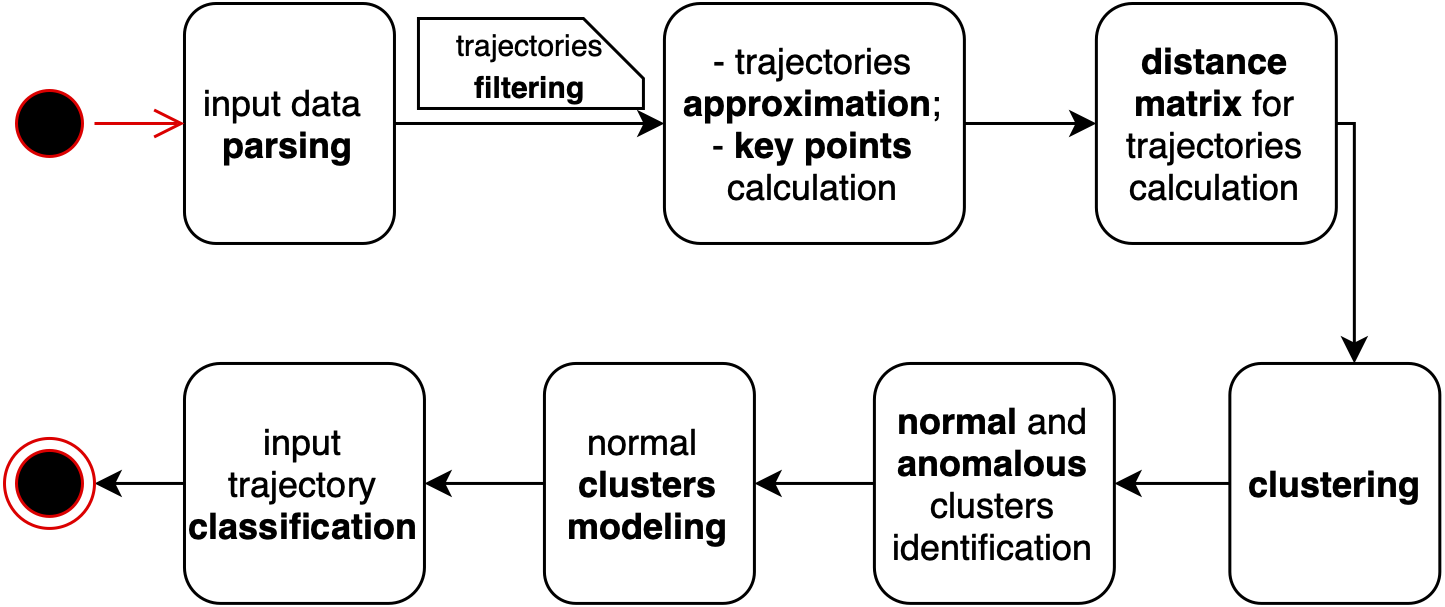
\includegraphics[width=0.8\textwidth]{images/flowchart.png}
	\caption{Основные этапы работы фреймворка}
	\label{fig:flowchart}
\end{figure}

\section{Архитектура фреймворка}

Архитектура предложенного подхода основана на работе \cite{inproceedings:7_related_work}, подробно описанной ранее, и состоит из двух частей (\ref{fig:str}):

\begin{itemize}
	\item \textit{offline} -- кластеризация и определние паттернов наиболее часто встречающихся траекторий, и
	\item \textit{online} -- классификация новой траектории как нормальной или аномальной.
\end{itemize}

\begin{figure}[!htb]
	\centering{}
	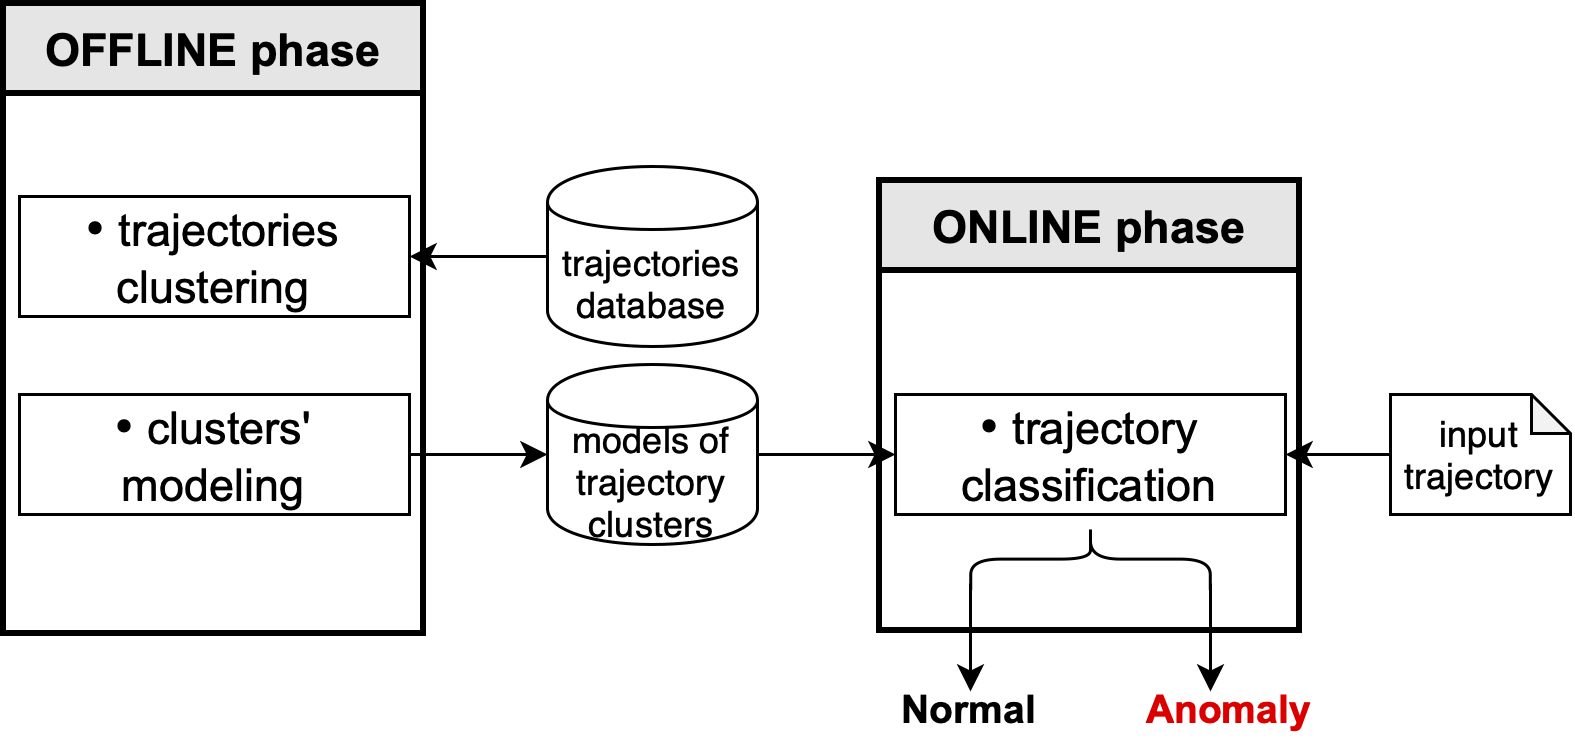
\includegraphics[width=0.8\textwidth]{images/str.png}
	\caption{Схема двухэтапного предложенного подхода}
	\label{fig:str}
\end{figure}

Фреймворк состоит из нескольких модулей, каждый из которых отвечает за выполнение одной из задач из вышеперечисленных этапов рабочего процесса (Figure \ref{fig:proj-arch}):
\begin{itemize}
	\item \textit{entity} -- содержит классы-сущности для хранения таких объектов, как $Trajectory$, $TrajectoryPoint$, $Cluster$ и др.;
	\item \textit{parsing} -- отвечает за парсинг входных данных: считывает данные из 'txt'-файла и создает объекты $TrajectoryPoint$ и $Trajectory$;
	\item \textit{csv} -- изолирует логику работы с 'csv'-файлами, содержит методы чтения и записи, которые используются сначала для сохранения подсчитанных LCSS метрик, а затем для их подгрузки для дальнейшей кластеризации;
	\item \textit{approximation} -- содержит реализацию аппроксимации траекторий методом полиномиальной регрессии и необходимые сопутствующие классы, такие как класс $Polynomial$, расширяющий функционал стандартного $PolynomialFunction$ из библиотеки Apache Math, и др.;
	\item \textit{visualization} -- отвечает за визаулизацию и сохранение полученных результатов, содержит методы для чтения, изменения, сохранения объектов класса $BufferedImage$;
	\item \textit{clustering} -- состоит из класса $Clustering$, который содержит методы для подсчета значений LCSS метрики, кластеризации объектов класса $Trajectory$ и создания объектов класса $Cluster$;
	\item \textit{exception} -- содержит исключения, которые теоретически могут быть выброшены в ходе работы фреймворка (например, $TrajectoryParserException$);
	\item \textit{misc} -- содержит вспомогательные утилитные классы для хранения константных значений и базовых методов, общих для всех модулей разрабатываемой системы.
\end{itemize}

\begin{figure}[!htb]
	\centering{}
	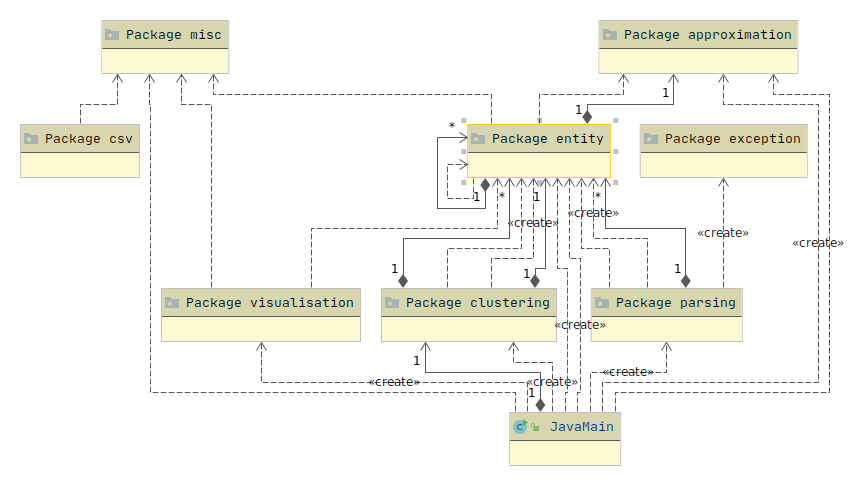
\includegraphics[width=0.8\textwidth]{images/proj-arch.png}
	\caption{Архитектура фреймворка}
	\label{fig:proj-arch}
\end{figure}

\section{Кластеризация}

\subsection{Агломеративная иерархическая кластеризация}

Для кластеризации был выбран агломеративный иерархический алгоритм кластеризации, работающий в режиме бесконтрольного обучения (unsupervised learning). Описание этого подхода приведено в алг. \ref{algo:ahc-descr} \cite{inproceedings:7_related_work}.

\begin{algorithm}[!htb]
	\caption{Описание Агломеративной Иерархической кластеризации}
	\label{algo:ahc-descr}
	\SetAlgoLined
	\KwIn{A Database of Trajectories: trajectories}
	\KwOut{Clusters of Trajectories: clusters}
	\textit{Initialization:} \\
	- initialize the clusters with one trajectory in each cluster \\
	\textit{Clusters merging:}\\
	\While{number of clusters is greater than 1}{
		- calculate similarity matrix D between pairs of clusters based on single linkage approach using LCSS similarity measure;\\
		- find the smallest distance between clusters in D;\\
		- merge two clusters with the corresponding smallest distance into a single cluster;\\
		- remove two merged clusters;\\
	}	
\end{algorithm}

Как уже упоминалось ранее, методы агломеративной иерархической кластеризации предполагают объединение кластеров, что требует определения меры расстояния между кластерами. В \cite{inproceedings:7_related_work} авторы провели сравнительный анализ различных связующих методов для определения схожести кластеров (linkage methods), включая single (метод связи по одной минимальной ссылке), maximum (метод связи по максимальнйо ссылке) и average (метод связи по средней ссылке) методы. Согласно проведенным тестам, single метод показал наилучшие результаты и поэтому будет использоваться в качестве метода связывания в текущей работе.

Метод связи по минимальной ссылке предполагает выбор минимального расстояния между двумя траекториями в качестве межкластерного расстояния и может быть представлен как \cite{inproceedings:7_related_work}:

\begin{equation} \label{eq:single_link}
D_{min}(C_i, C_j) = \min_{T_1 \in C_i, T_2 \in C_j} D_{LCSS}(T_1, T_2),
\end{equation} 

где ($C_i$, $C_j$) обозначают два кластера, а ($T_1$, $T_2$) соответствуют двум траекториям из двух кластеров соответственно.

\subsection{Моделирование кластеров}

Чтобы более эффективно выполнить дальнейшую классификацию входной траектории, в выбранной в качестве основы работе было предложено создать модели кластеров (модели траекторий), классифицированных как нормальные. Моделью кластера называется ее компактное представление. Модели нормальных кластеров можно рассматривать как шаблоны частых траекторий, поскольку они представляют собой весь кластер траекторий с максимальной точностью.

Существуют две основные концепции построения модели кластера \cite{article:surv_cl_models}:
\begin{itemize}
	\item выбор репрезентативной траектории из кластера. Такая траектория считается центром кластера. Самым простым способом обозначить репрезентативную траекторию является определение только ее центроида (центроид кластера, путь центроида). В качестве дополнения центроид может быть расширен определением диапазона, области пути центроида;
	\item определение модели на основании траекторий, относящихся к кластеру, с использованием вероятностных моделей, таких как Гауссовские наблюдательные эмиссионные HMM (Hidden Markov Model). Такой метод требует предварительной обработки траекторий и показвыает лучшие результаты на вероятностно моделируемых траекториях.
\end{itemize}

По сравнению со второй концепцией, выбор репрезентативной траектории для каждого кластера в качестве модели является более простым методом. Более того, он не требует, чтобы траектории имели одинаковое количество точек траектории \cite{inproceedings:7_related_work}.

Авторы \cite{inproceedings:7_related_work} предлагают легкий подход к моделированию кластера без какой-либо предварительной обработки траекторий: модель кластера - это траектория, наименее всего удаленная от других, в результате чего ее можно рассматривать как репрезентативный центр кластера. Это означает, что необходимо определить траекторию с минимальным средним расстоянием LCSS до других траекторий в этом кластере (\ref{eq:cm_traj}):

\begin{equation} \label{eq:cm_traj}
	CM(C) = \min\limits_{T \in C} \frac{1}{|C|} \sum_{T' \in C} D_{LCSS}(T, T')
\end{equation}

\section{Сравнение траекторий}

Для измерения схожести и расстояния между траекториями для выполнения кластеризации в этой работе будет использоваться LCSS расстояние. LCSS расстояние подразумевает вычисление самой длинной общей подпоследовательности между двумя входными траекториями с использованием двух значений параметров: $\delta$ и $\varepsilon$.

\subsection{LCSS метрика для измерения схожести траекторий}

Согласно методу LCSS, параметры $\delta$ и $\varepsilon$ являются постоянными и задаются заранее. Однако в текущем предлагаемом подходе для работы с неопределенностью данных о траектории, содержащих точки траектории, расположенные произвольным образом по отношению к камере, было решено реализовать адаптивность значений параметров. Будет исследована функциональная зависимость параметров от положения движущегося объекта на перекрестке относительно камеры.

При визуальном анализе траекторий, отображенных на исходных изображениях с камер, можно сделать несколько выводов: поскольку нижняя часть изображения представляет область, расположенную ближе к камере наблюдения, движущиеся объекты в верхней части изображения более отдалены от камеры, и в результате более плотно расположены относительно друг друга на изображении. $\varepsilon$ представляет собой пороговую величину, регулирующую пространственную удаленность точек траектории при подсчете расстояния между ними. Следовательно, он должен быть адаптирован к удаленности и уменьшаться по мере удаления точки траектории от камеры.

Описание алгоритма подсчета LCSS приведено в алг. \ref{algo:lcss-descr}.

\begin{algorithm}[!htb]
	\caption{Описание алгоритма LCSS метрики}
	\label{algo:lcss-descr}
	\SetAlgoLined
	\KwIn{First trajectory: $T_1$,\newline
			Second trajectory: $T_2$,\newline
			Temporal remoteness threshold: $\delta$,\newline
			Spatial remoteness threshold: $\varepsilon$
	}
	\KwOut{LCSS distance for two trajectories}
	\Begin{
		// Initialization \\
		- calculate length of $T_1$\;
		- calculate length of $T_2$\;
		// LCSS similarity calculation \newline	
		\eIf {$T_1$ or $T_2$ is empty}{
			return 0;	
		}{\eIf {difference between X-coordinates < $\varepsilon$ \newline
			AND difference between Y-coordinates < $\varepsilon$ \newline
			AND difference between trajectory lengths < $\delta$}{
				- increase LCSS by 1\;
				- call recursive for trajectories excluding last points\;
			}{
				- calculate LCSS for first trajectory and second trajectory 	excluding last point\;
				- calculate LCSS for first trajectory excluding last point and second trajectory\;
				- take maximum between these LCSS values\;
			}
		}
		// LCSS distance calculation \\
		LCSS distance = 1 - LCSS similarity / minimum(input lengths)
	}
\end{algorithm}

\subsection{Адаптивность параметров LCSS алгоритма}

Классический метод подсчета LCSS предполагает использование постоянных значений для параметров $\delta$ и $\varepsilon$ и не подразумевает их адаптивности. Тем не менее, одной из целей в этой работе является исследование возможности повышения точности результатов путем изучения функциональной зависимости между этими параметрами и удаленностью движущейся точки от камеры.

По причине того что камера расположена в фиксированном месте на перекрестке, возможны проблемы, связанные с перспективой. Из рис. \ref{fig:tr_p}, на котором изображено распределение исходных траекторий, видно, что при удалении от камеры, расположенной в нижней передней части изображения, траектории становятся более плотно расположенными относительно друг друга ( входные данные будут описаны и изображены в следующей главе). В случае константного значения $\varepsilon$, контролирующего допустимое пространственное отклонение между точками траектории при тестировании пространственного равенства точек траектории, точки траектории, расположенные далеко от камеры (то есть появляющиеся в верхней части изображений с камер и расположенные более плотно друг к другу), будут неправильно признаны похожими. Это может негативно повлиять на последующий анализ и исказить дальнейшие результаты кластеризации.

Следовательно, значение коэффициента $\varepsilon$ должно меняться в соответствии с расстоянием от местоположения камеры: $\varepsilon$ должен уменьшаться по мере удаления точки траектории от камеры и увеличиваться по мере приближения точки траектории к камере. Таким образом, можно предположить, что $\varepsilon$ и расстояние от камеры находятся в обратной зависимости, что означает, что в итоговой формуле расстояние от камеры должно присутствовать в знаменателе формулы с некоторым коэффициентом.

Подход к определению адаптивных параметров, рассмотренный в данной работе, описан в алг. \ref{algo:lcss-params-adapt} и изображен на рис. \ref{fig:adaptability}.

\begin{algorithm}[!htb]
	\caption{Определение адаптивных параметров LCSS}
	\label{algo:lcss-params-adapt}
	\SetAlgoLined
	\KwIn{First trajectory point: $TP_1$,\newline
		Second trajectory point: $TP_2$
	}
	\KwOut{Adaptive $\varepsilon$ value for $TP_1$ and $TP_2$}
	\Begin{
		// Initialization \\
		- compute location of a camera point ($CP$)\;
		- compute Euclidean distance for two pairs $d_1$($TP_1$, $CP$) and $d_2$($TP_2$, $CP$)\;
		- compute corresponding $\varepsilon_1$ and $\varepsilon_2$ values\;
		- take the $\max(\varepsilon_1,\ \varepsilon_2)$ as a final $\varepsilon$ to compare $TP_1$ and $TP_2$.
	}
\end{algorithm}

\begin{figure}[!htb]
	\centering{}
	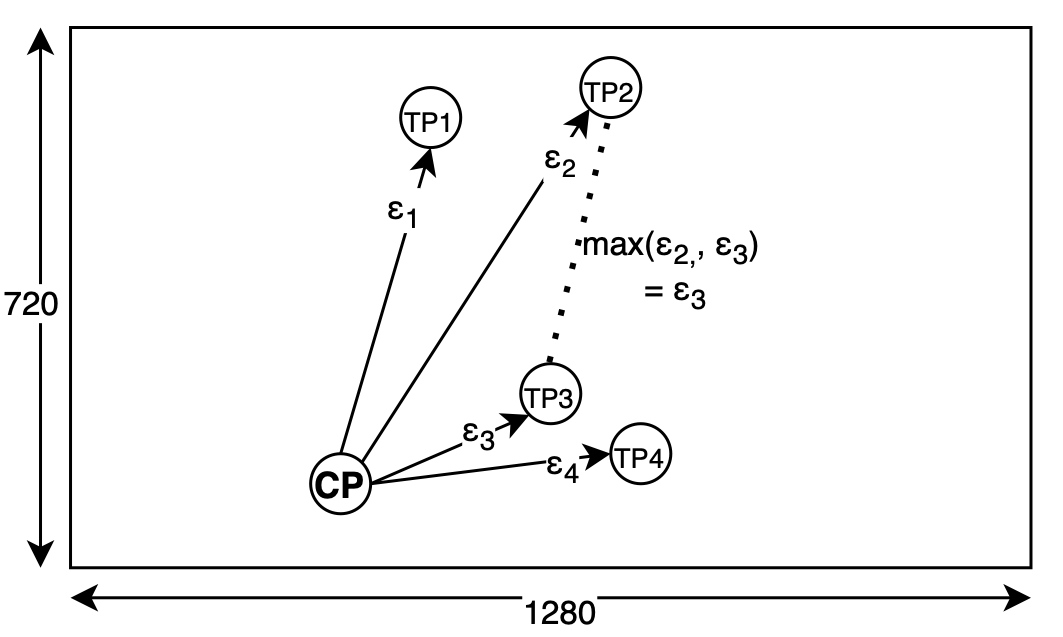
\includegraphics[width=0.7\textwidth]{images/adaptivity.png}
	\caption{Принцип выбора адаптивного значения $\varepsilon$}
	\label{fig:adaptivity}
\end{figure}

Чтобы оптимизировать подсчет расстояния от точки траектории до точки камеры и избежать его многократного пересчета во время работы алгоритма вычисления LCSS, это расстояние рассчитывается заранее и сохраняется для каждой точки траектории.

\section{Проверка достоверности кластеров}

Поскольку целью настоящей работы является поиск оптимальных значений адаптивных параметров для вычисления метрики сходства траекторий, необходимо проанализировать и сравнить полученные результаты после выполнения кластеризации.

Согласно \cite{online:dunn_cl_valid} метрики проверки достоверности результатов кластерного решения могут быть классифицированы следующим образом:
\begin{itemize}
	\item \textbf{Internal cluster validation} -- внутренняя метрика оценки кластеров. Результат кластеризации оценивается на основе кластеризованных входных данных. Он основан на внутренней информации и не содержит ссылок на внешнюю информацию.
	\item \textbf{External cluster validation} -- внешняя метрика оценки кластеров. Оценка результатов кластеризации выполняется в соответствии с известными извне результатами, например, данными метками класса. Такая проверка не подходит для неконтролируемой (unsupervised) кластеризации, поскольку в таком случае входные метки неизвестны.
	\item \textbf{Relative cluster validation} -- относительная метрика оценки кластеров. Оценка результатов кластеризации выполняется с помощью одного и того же алгоритма с использованием разных входных параметров, таких как количество кластеров и т.д..
\end{itemize}

В то же время кластеризация - это, прежде всего, метод бесконтрольного неконтролируемого извлечения данных, использующий входные данные, не содержащие меток данных. Это приводит к необходимости проверять итоговые кластеры неконтролируемым образом.

Одной из наиболее широко используемых и известных метрик для оценки алгоритмов кластеризации является индекс достоверности Данна (Dunn's Validity Index, DI), который был предложен Дж. К. Данном в 1974 году в \cite{article:dunn_orig}. Это внутренняя метрика оценки, предназначенная для идентификации компактных кластеров с небольшой дисперсией между элементами кластера, которые хорошо отделены друг от друга, то есть кластеры достаточно отдалены от окружающих кластеров по сравнению с межкластерной дисперсией \cite{online:hier_clust_r}. DI рассчитывается как отношение минимального межкластерного расстояния $d_{min}$ к максимальному внутрикластерному диаметру $d_{max}$, и для $k$ кластеров может быть определен следующим образом (\ref{eq:dunn-index}) \cite{article:quant_eval_perf_clust}:

\begin{equation} \label{eq:dunn-index}
	DI = \frac {d_{min}} {d_{max}} = \frac{\min\limits_{\substack{1 \leq i \leq k \\ i+1 \leq j \leq k}} dist(c_i, c_j)} {\max\limits_{1 \leq l \leq k} diam(c_l)}
\end{equation}

где минимальное межкластерное расстояние $d_{min}$ в соответствии с методом связи по минимальной ссылке сводится к подсчету минимального расстояния между двумя траекториями из разных кластеров. Максимальный внутрикластерный диаметр $d_{max}$, или самое большое внутрикластерное расстояние, предполагает вычисление диаметра кластера как расстояния между его двумя самыми дальними траекториями \cite{inproceedings:clust_ind}.

Пример определения DI для 3 кластеров приведен на рис. \ref{fig:di_sample}. Согласно этому примеру (\ref{eq:dunn-index-sample}) может быть переписан следующим образом:

\begin{equation} \label{eq:dunn-index-sample}
DI = \frac {d_{min}} {d_{max}} = \frac
	{\min ({dist_{min}}^1, {dist_{min}}^2, {dist_{min}}^3)}
	{\max ({diam_{max}}^1, {diam_{max}}^2, {diam_{max}}^3)}
\end{equation}

\begin{figure}[!htb]
	\centering{}
	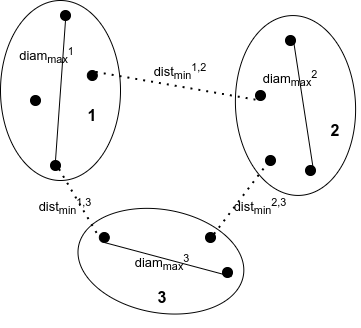
\includegraphics[width=0.5\textwidth]{images/di-sample.png}
	\caption{Объяснение индекса DI}
	\label{fig:di_sample}
\end{figure}

Более высокие значения DI указывают на лучшие результаты кластеризации. Траектории, расположенные далеко друг от друга внутри одного кластера, должны отличаться от траекторий, относящихся к другим кластерам. Близкие к 1 значения DI означают, что минимальные расстояния до траекторий из разных кластеров остаются больше, чем расстояние до самых дальних траекторий внутри одного кластера. Однако вычислительная стоимость DI сильно зависит от данных: вычислительная сложность увеличивается с ростом количества кластеров и размерности данных \cite{online:dunn_cl_valid}.

\section{Аппроксимация траекторий}

Несмотря на то что метрика подобия LCSS работает с траекториями произвольных длин и по умолчанию не требует предварительной обработки траекторий, подсчет LCSS метрики становится чрезвычайно вычислительно сложным и времязатратным с ростом длины траектории в результате рекурсивности. По этой причине в текущей работе было решено уменьшить размер траекторий путем аппроксимации исходных траекторий. Это приводит к потере точности, но позволяет получить приемлемые результаты за адекватное количество времени.

Концепция подбора аппроксимирующей кривой функции - это один из стандартных подходов для выполнения аппроксимации \cite{article:behav_form_extr}. Основная задача - найти подходящее соотношение или закон, возможно существующий между входными (независимыми) и выходными (зависимыми) переменными для заданного набора входных данных наблюдаемых значений. И подбор кривой - это процесс выражения связи между переменными в терминах алгебраических уравнений. Основная цель подбора кривой - найти параметры для модели (уравнения или функции), подходящей для экспериментальных данных.

\subsection{Регрессионный анализ}

Одним из наиболее широко используемых подходов, основанных на концепции подбора кривой, является регрессионный анализ, который также рассматривается как форма подхода прогнозирующего моделирования и, согласно традиционному определению, изучает взаимосвязь между зависимой переменной (результатом) $Y$ и одним или более независимыми переменными $X$ и, как правило, находит тренды в данных. Другими словами, он предполагает «использование отношения между переменными для подбора линии наилучшего соответствия или уравнения регрессии, которое можно использовать для прогнозирования» \cite{online:intro_lr_pr}.

С целью упростить процедуру подбора аппроксимирующей функции обычно предполагается, что независимые переменные $X$ измеряются без ошибок, в то время как значения зависимых переменных $Y$ измеряются с некоторой случайной ошибкой. Для данных с небольшим отношением ошибки измерения в независимой переменной к диапазону значений этой переменной можно правомерно использовать регрессионный анализ по методу наименьших квадратов \cite{article:behav_form_extr}.

Регрессия может быть линейной или полиномиальной (нелинейной, криволинейной) в зависимости от функции, которая аппроксимирует данные: линейная регрессия применима к отношениям, аппроксимируемым прямой линией, тогда как криволинейная регрессия относится к отношениям,  аппроксимируемым кривой. Благодаря более широкому диапазону функций, с которыми может работать полиномиальная регрессия, она обеспечивает лучшее приближение входных отношений по сравнению с линейной регрессией \cite{online:intro_lr_pr}. Даже если невозможно заранее определить тип функции для аппроксимации, чтобы получить наивысшую точность результатов, может оказаться полезным визуализация и анализ отображения исходных данных для нахождения какого-либо поведенческого паттерна, такого как линейная, квадратичная или зависимость более высокого порядка \cite{article:behav_form_extr}.

\subsection{Полиномиальная регрессия}

Визуализация исходных данных траекторий представлена на рис. \ref{fig:tr_p}. Как видно из рисунка, ни линейные функции, ни функции $2$-го порядка не могут соответствовать данным должным образом из-за сложности форм траектории. По этой причине было решено сосредоточиться на приближении с использованием полиномиальной регрессии высшего порядка. Оценка полиномиальной регрессии с различными степенями будет приведена далее, и последующее обсуждение и реализация будут направлены на то, чтобы найти подходящее полиномиальное уравнение $n$-го порядка со значениями параметров для представления каждой входной траектории в качестве «функции траектории». Поскольку данные траектории представлены двумерными пространственными данными вместе с временными данными, и необходимо аппроксимировать пространственную информацию, $x$- и $y$ -координаты будут рассматриваться как зависимые переменные, а $time$ будет использоваться как независимая переменная. Следовательно, полиномиальная регрессия будет выполняться дважды с двумя выходными полиномиальными функциями, представляющими $x(t)$ и $y(t)$ для каждой из входных траекторий $T$:

\begin{equation}\label{eq:regr-func}
	\forall\ T = [\ldots (x_i, y_i, t_i) \ldots] = > T(t) = 
		\begin{cases}
			x = x(t) \\
			y = y(t) \\
		\end{cases}
\end{equation}

Таким образом, траектории будут преобразованы из формата списка точек траекторий в уравнения (функции времени), определенные в геометрическом пространстве, которые могут с высокой точностью представлять все исходные траектории. Выбор ключевых точек репрезентативного полинома может уменьшить размер траектории, тем самым сокращая итоговые эксплуатационные затраты и вычислительную сложность LCSS. Кроме того, математические уравнения способны хранить информацию в плотной форме, и, помимо других преимуществ, такое сокращение данных приводит к уменьшению занимаемого пространства и повышению эффективности хранения \cite{article:behav_form_extr}. Также так называемые встроенные «функции траектории» могут обеспечивать интерполяцию и позволяют определять пропущенные, потерянные точки траекторий.
 		% Framework Conceptual Model (Suggested Approach)
\chapter{РЕАЛИЗАЦИЯ ФРЕЙМВОРКА}
\label{ch:РЕАЛИЗАЦИЯ ФРЕЙМВОРКА}

В этой главе дается описание разработки фреймворка с предоставлением деталей реализации описанной ранее концепции на базе выбранного стека технологий. На основе изложенного ранее рабочего процесса фреймворка были реализованы отдельные модули, подробное описание каждого из них представлено в следующих разделах. Первые разделы описывают обработку и аппроксимацию входных данных траектории. В последующих разделах представлены детали реализации решения задач кластеризации, моделирования кластеров и классификации входных траекторий. По причине того что не было найдено подходящих готовых реализаций для выбранных алгоритмов, все реализации алгоритмов, кроме полиномиальной регрессии и решения полиномиальных уравнений, были написаны с нуля и представлены в Приложениях.

\section{Используемые технологии}

Для реализации фреймворка был выбран язык программирования Java с сопутствующими библиотеками и Apache Maven в качестве инструмента для автоматизации сборки для проектов Java следующих версий:

\begin{itemize}
	\item Java - 11 OpenJDK
	\item Apache Maven - 3.6.3
	\item Commons Math: The Apache Commons Mathematics Library - 3.4.1
	\item Java AWT, Javax Swing 
\end{itemize}

Java используется как основной язык программирования. Библиотека Commons Math library была выбрана для реализации аппроксимации траекторий, поскольку она предлагает реализацию для таких классов, как $PolynomialFunction$ и $PolynomialSolver$. 

Java AWT (Abstract Window Toolkit) представляет собой ИПП (Интерфейс прикладного программирования, API) для реализации ГПИ (Графический Пользовательский Интерфейс, GUI) в Java приложениях и поставляется как часть Java JDK начиная с версии OpenJDK 7. В данной работе Java AWT будет использоваться преимущественно для создания и манипуляции объектами $BufferedImage$ для визуализации исходных изображений с камер и отображения траекторий на них.

Java Swing, так же как и Java AWT, является инструментальной библиотекой, созданной для тех же целей предоставления ГПИ приложениям, написанным на Java, и реализации возможности написания приложений, основанных на применении окон (оконных приложений). Однако Swing является более новой и продвинутой библиотекой, поддерживающей более сложные, усовершенствованные ГПИ-компоненты, нежели Java AWT. В текущей работе Swing используется для создания окон для визуализации изображений с исходными траекториями, результатами аппроксимации и кластеризации.

\section{Описание входных данных}

Согласно исследованию, проведенному Министерством транспорта США на основе данных Системы отчетов об анализе смертности (Fatality Analysis Reporting System, FARS) и Национальной системы отбора проб автомобилей (National Automotive Sampling System), почти 40 процентов всех зарегистрированных в 2008 году аварий произошли на перекрестках \cite{inproceedings:10_cfi}. Следовательно, в настоящее время анализ транспортной активности на перекрестках на перекерстках дорог имеет большое значение в контексте безопасности, и выявление небезопасных транспортных траекторий, нарушающих ПДД, может быть одним из шагов на пути к улучшению статистики.

В представленной работе видео с камер слежения используется для обучения и тестирования системы. Тестовые видео получены с помощью ИТС, реализованных и установленных на четырех перекрестках в г. Казань:

\begin{enumerate}
	\item Перекресток улиц Право-Булачная - Пушкина, $1.txt$ (рис. \ref{fig:is_1}).
	\item Перекресток улиц Несмелова - Кировская Дамба, $2.txt$ (рис. \ref{fig:is_2}).
	\item Перекресток улиц Московская - Галиаскара Камала, $3.txt$ (рис. \ref{fig:is_3}).
	\item Перекресток улиц Московская - Парижской Коммуны, $4.txt$ (рис. \ref{fig:is_4}).
\end{enumerate}

Каждый перекресток представляет собой четырехстороннее пересечение дорог, оборудованное одной регистрирующей камерой. Примеры изображений с установленных видеокамер представлены на рис. \ref{fig:is_all}.

\begin{figure}[!htb]
	\centering
	\begin{subfigure}[!htb]{0.48\textwidth}
		\centering{}
		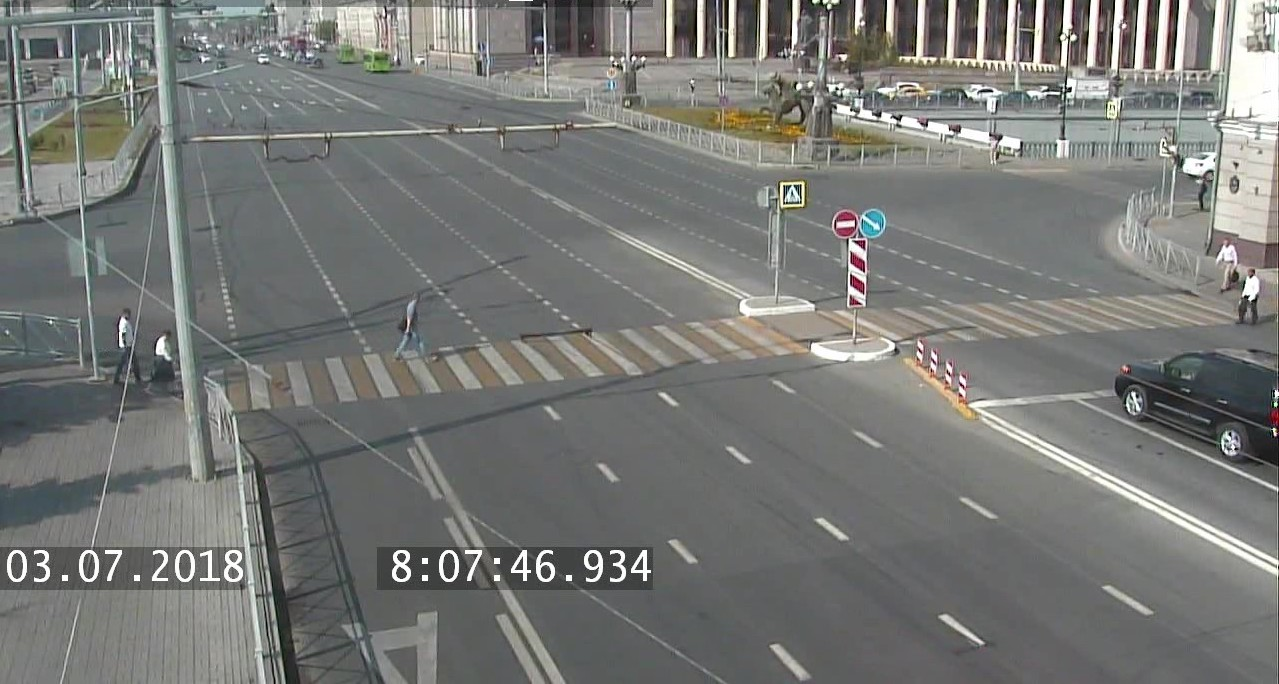
\includegraphics[width=\textwidth]{images/is-1.jpg}
		\caption{$1.txt$}
		\label{fig:is_1}
	\end{subfigure}
	\hfill
	\begin{subfigure}[!htb]{0.48\textwidth}
		\centering{}
		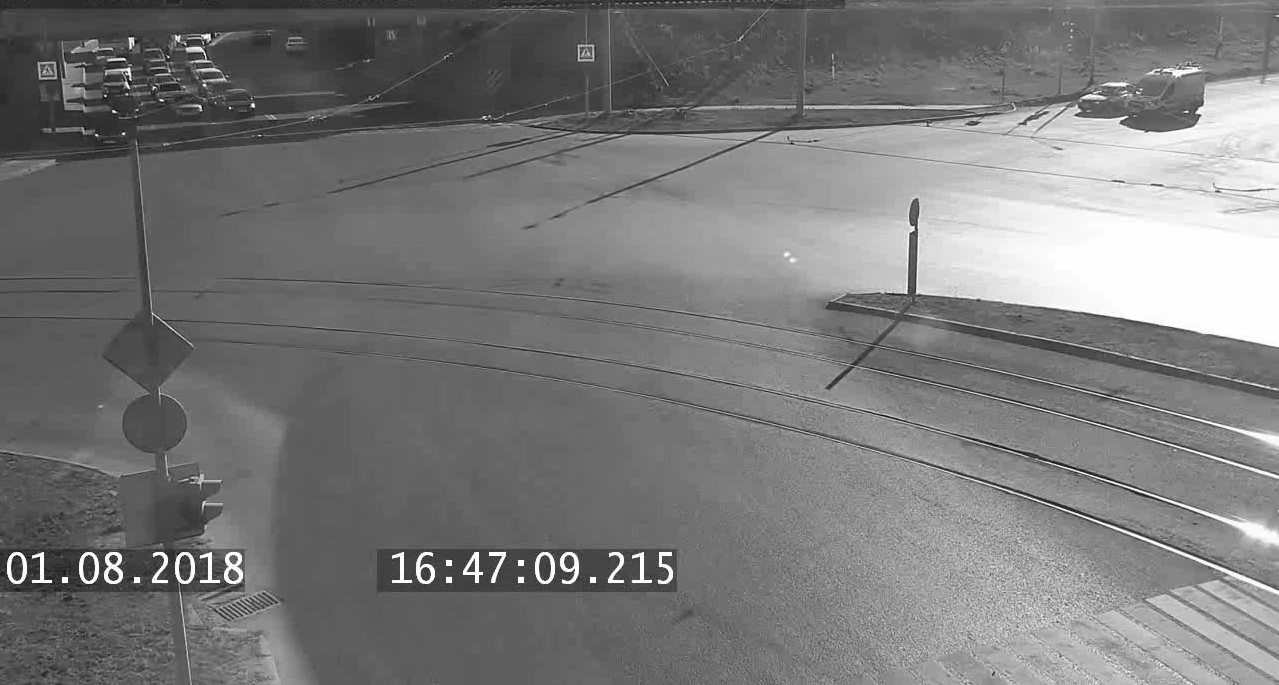
\includegraphics[width=\textwidth]{images/is-2.jpg}
		\caption{$3.txt$}
		\label{fig:is_2}
	\end{subfigure}
	\hfill
	\begin{subfigure}[!htb]{0.48\textwidth}
		\centering{}
		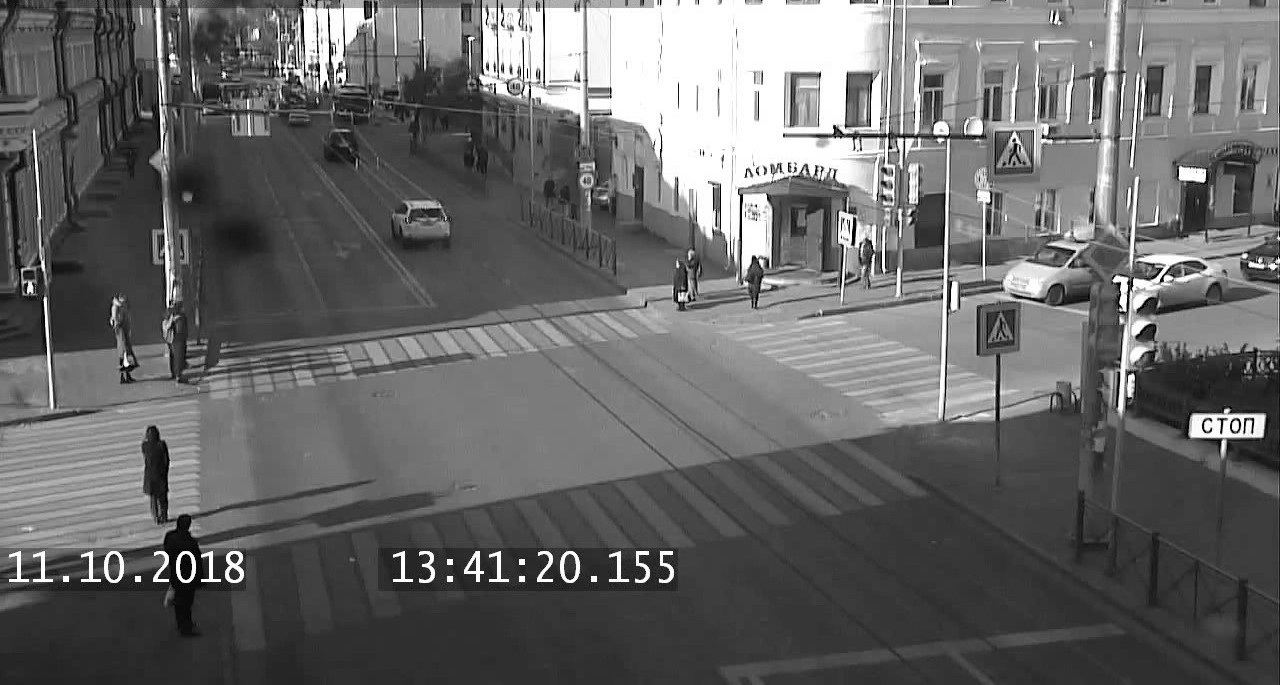
\includegraphics[width=\textwidth]{images/is-3.jpg}
		\caption{$4.txt$}
		\label{fig:is_3}
	\end{subfigure}
	\hfill
	\begin{subfigure}[!htb]{0.48\textwidth}
		\centering{}
		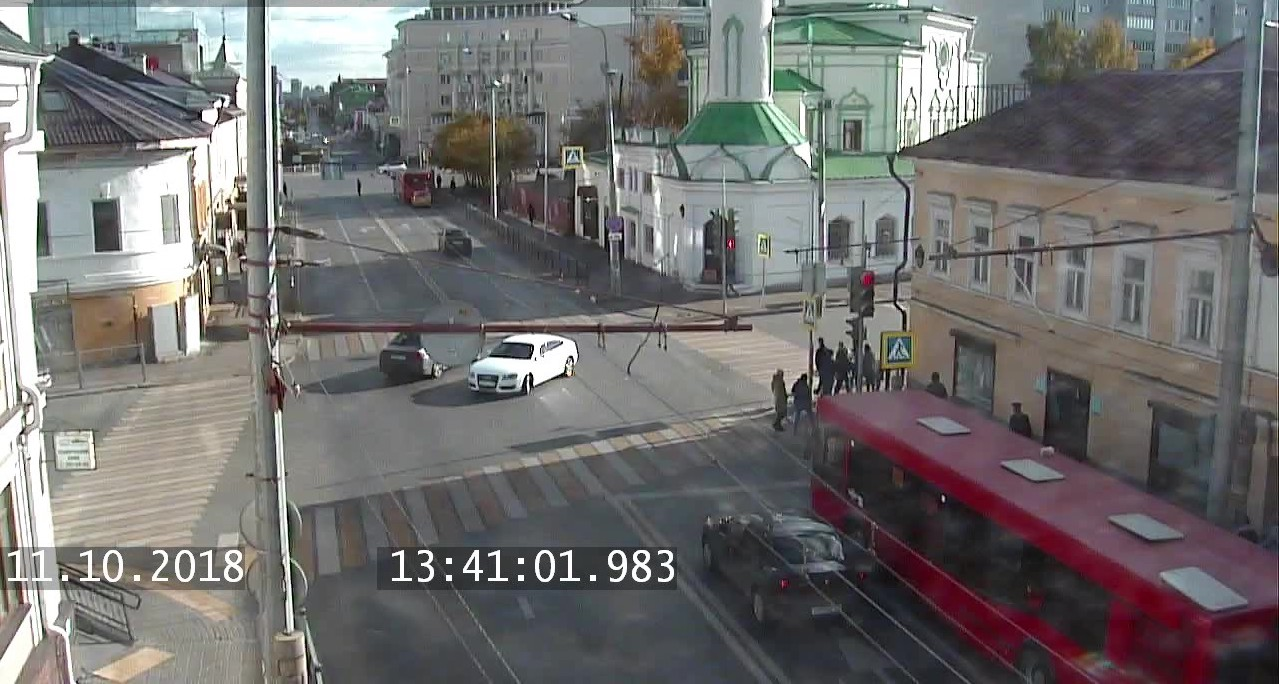
\includegraphics[width=\textwidth]{images/is-4.jpg}
		\caption{$4.txt$}
		\label{fig:is_4}
	\end{subfigure}
	\caption{Примеры изображений с видеокамер на перекрестках 1-4}
	\label{fig:is_all}
\end{figure}

Файлы с входными данными содержат 624, 211, 231, 237 траекторий ТС для каждого из указанных перекрестков соответственно.

Под аномальной траекторией подразумевается траектория движения ТС через перекресток, которая значительно отличается от большинства известных, нормальных траекторий. Например, в случае, когда на перекрестке запрещен поворот направо с крайней левой полосы движения, такое поведение будет неизвестно системе. В случае появления такой траектории она будет признана системой аномальной.

\begin{figure}[!htb]
	\centering{}
	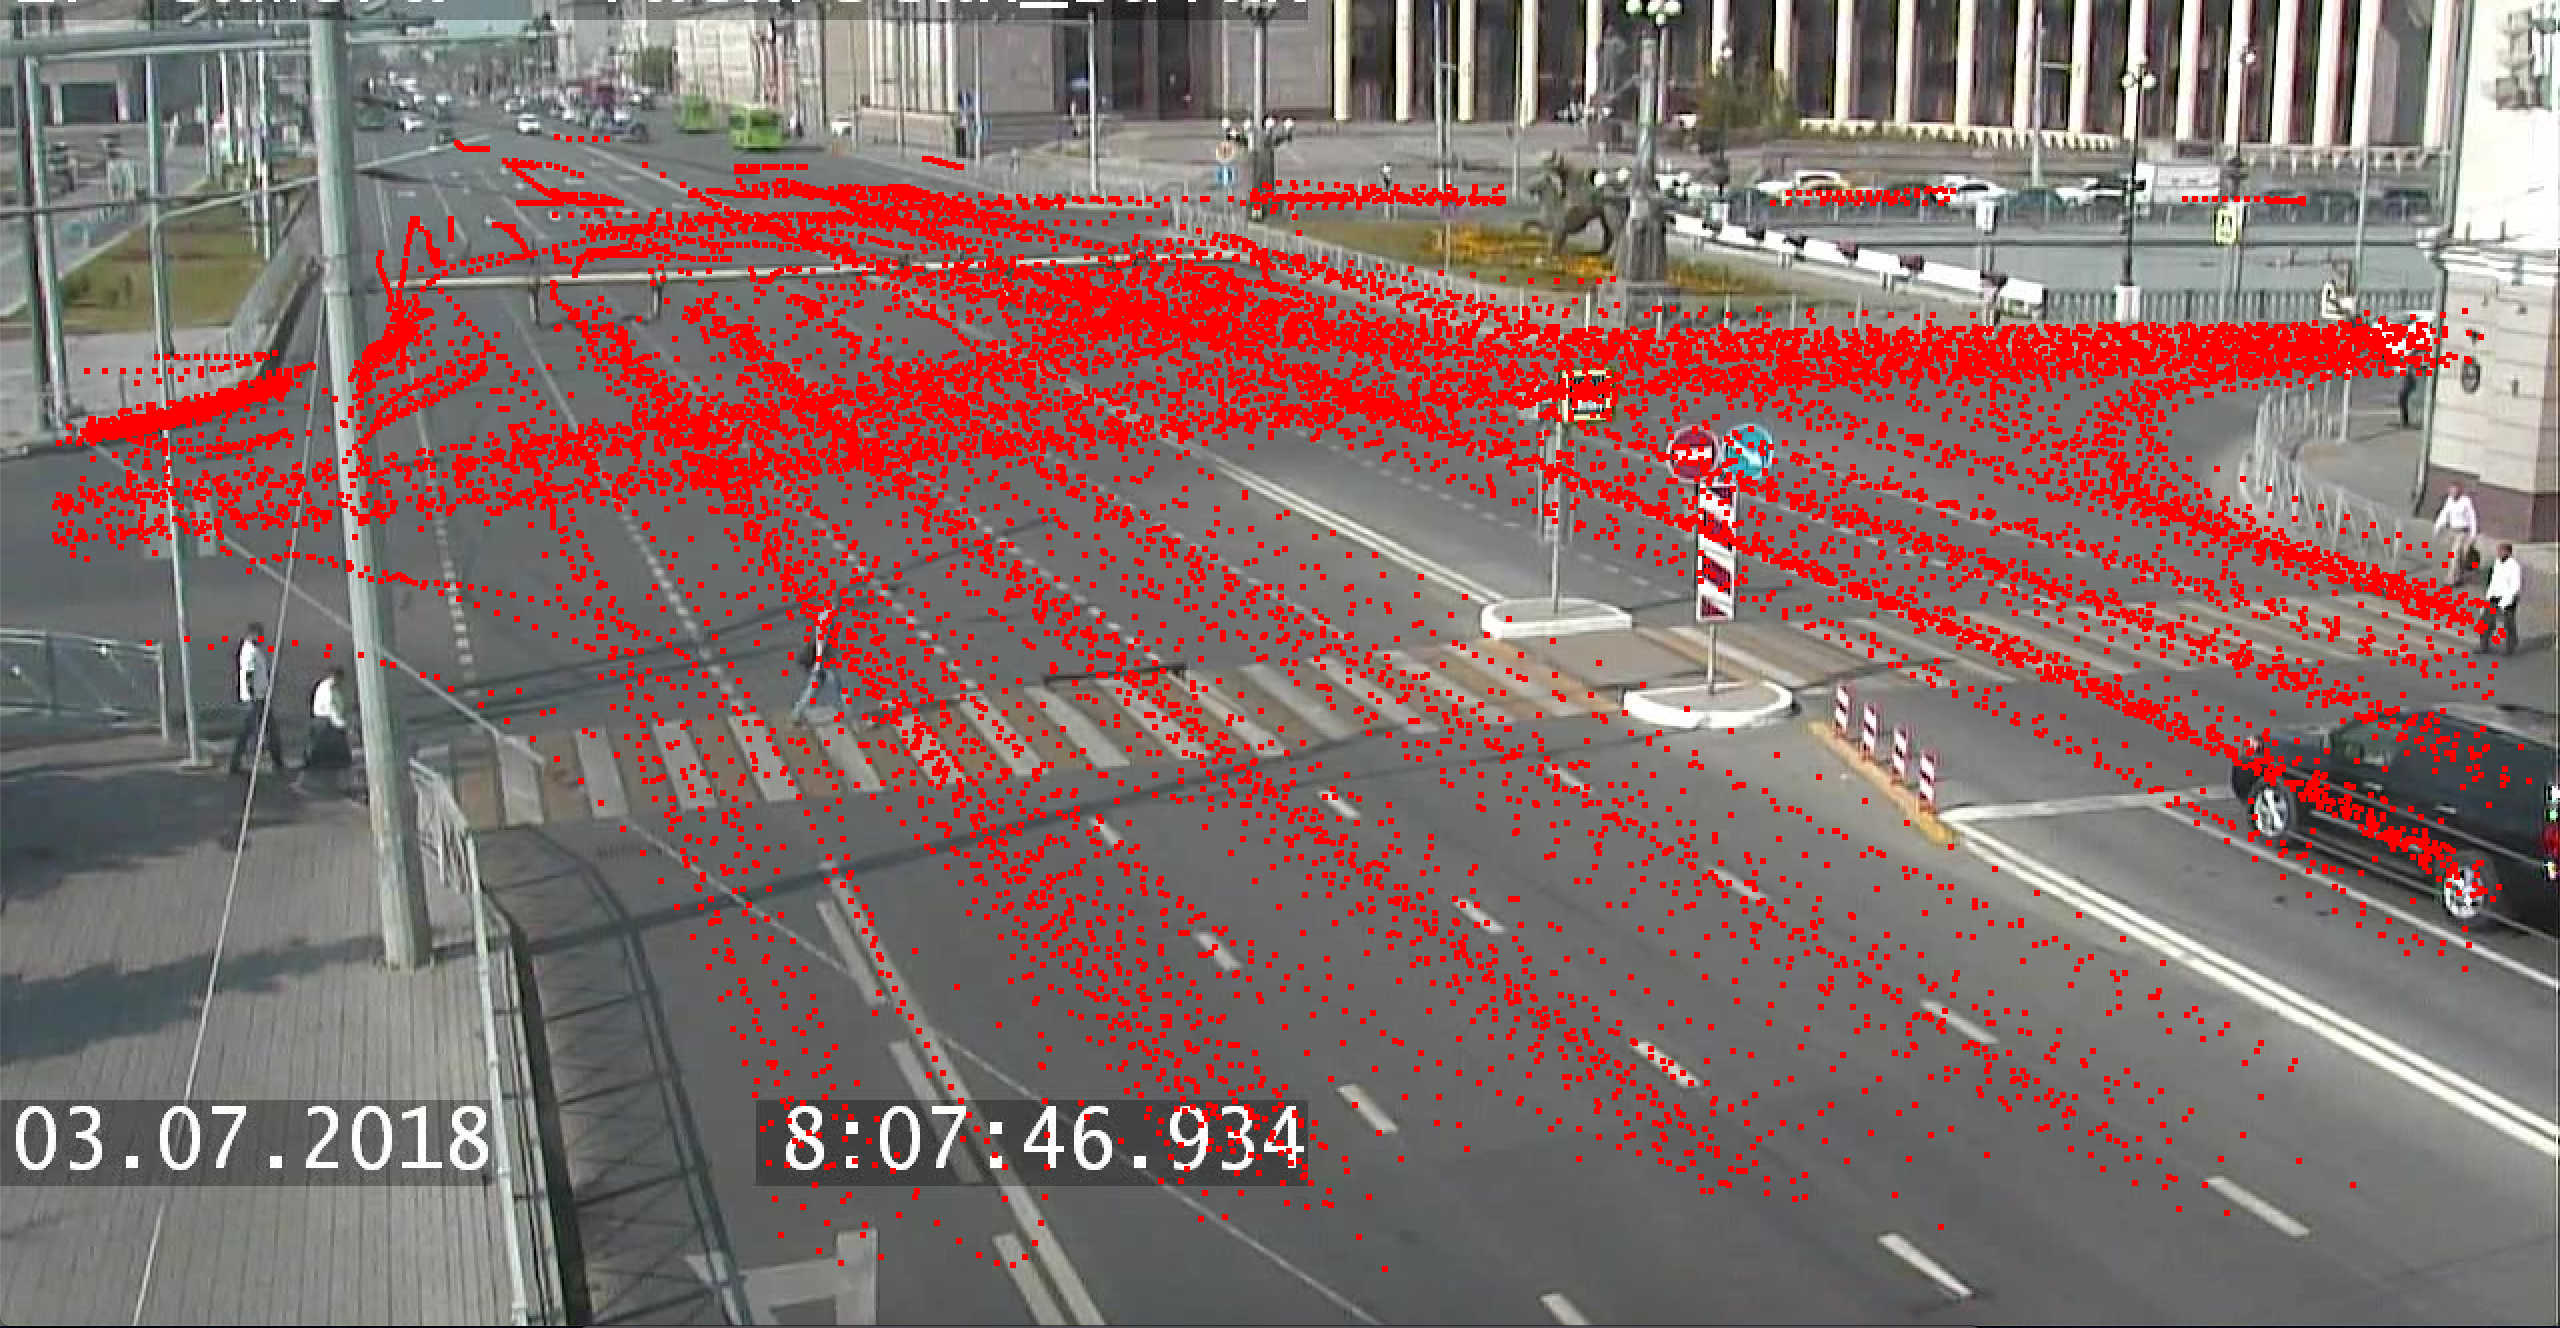
\includegraphics[width=0.8\textwidth]{images/tr-p.png}
	\caption{Пример работы системы слежения на данных с первого перекрестка}
	\label{fig:tr_p}
\end{figure}

\subsection{Структура файла входных данных}

Система отслеживания, как было описано ранее, обрабатывает видео с камер слежения и подготавливает его для дальнейшего анализа: преобразует видеопоток в набор векторов с точками отслеживания (далее точки траектории) на изображениях (рис. \ref{fig:tr_p}).

Файлы входных данных имеют следующую структуру:

\begin{equation} \label{eq:input_str}
[[[(x_1^1, y_1^1), ..., (x_1^n, y_1^n)], [t_1, ... t_n]], [[(x_2^1, y_2^1), ..., (x_2^m, y_2^m)], [t_1, ... t_m]], ...]
\end{equation}

Как видно из структуры файла входных данных, каждая траектория представлена двухэлементным массивом, где первый массив хранит координаты в виде массива пар $(x_i^j, y_i^j)$, а второй массив содержит временные метки для каждой пространственной точки в соответствующем порядке $(t_i)$. Извлеченные координаты $x$ и $y$ соответствуют пикселям на входных изображениях. В формуле \ref{eq:input_str} нижний индекс пространственных координат указывает на порядковый номер траектории, а верхний индекс представляет собой порядковый номер точки отслеживания. Внешний массив является массивом траекторий.

\section{Обработка входных данных}

Поскольку выбранный алгоритм ожидает получить траектории в виде многомерных векторов, исходные входные данные необходимо преобразовать к подходящему формату. Для этих целей был реализован пользовательский парсер, принимающий текстовый файл ``txt'' с траекториями в указанном ранее формате в качестве входных данных и в результате возвращающий список объектов $Trajectory$. Объект $Trajectory$ состоит из нескольких объектов $TrajectoryPoint$ со следующими атрибутами: \textit{x}-координата, \textit{y}-координата, время \textit{t}. Исходный код метода синтаксического анализа приведен в Приложении А.

Входные данные содержат траектории различной длины и с различным пройденным расстоянием. Однако из-за неточности и ошибок в системе слежения некоторые траектории выглядят неправдоподобно и не имеют смысла. Одна из возможных причин этого - пропавший отслеживаемый объект или потеря системой слежения местоположения объекта. В отличие от случая потерянного местоположения, когда пропущенное местоположение может быть найдено с использованием моделей аппроксимации и регрессии, потерянный объект отслеживания не может быть впоследствии исправлен. По этой причине, чтобы улучшить качество результатов, было решено отфильтровать входные траектории и игнорировать короткие траектории с малым пройденным расстоянием, где пройденное расстояние рассчитывается как евклидово расстояние между первой и последней точками траектории. Для фильтрации параметров использовались следующие значения: $minLength = 10\ (trajectory \ points)$, $minTotalDist = 80 \ (pixels)$. Результаты фильтрации с отображением удаленных и сохраненных траекторий показаны на рис. \ref{fig:traj_filter}.

\begin{figure}
	\centering
	\begin{subfigure}[b]{0.48\textwidth}
		\centering{}
		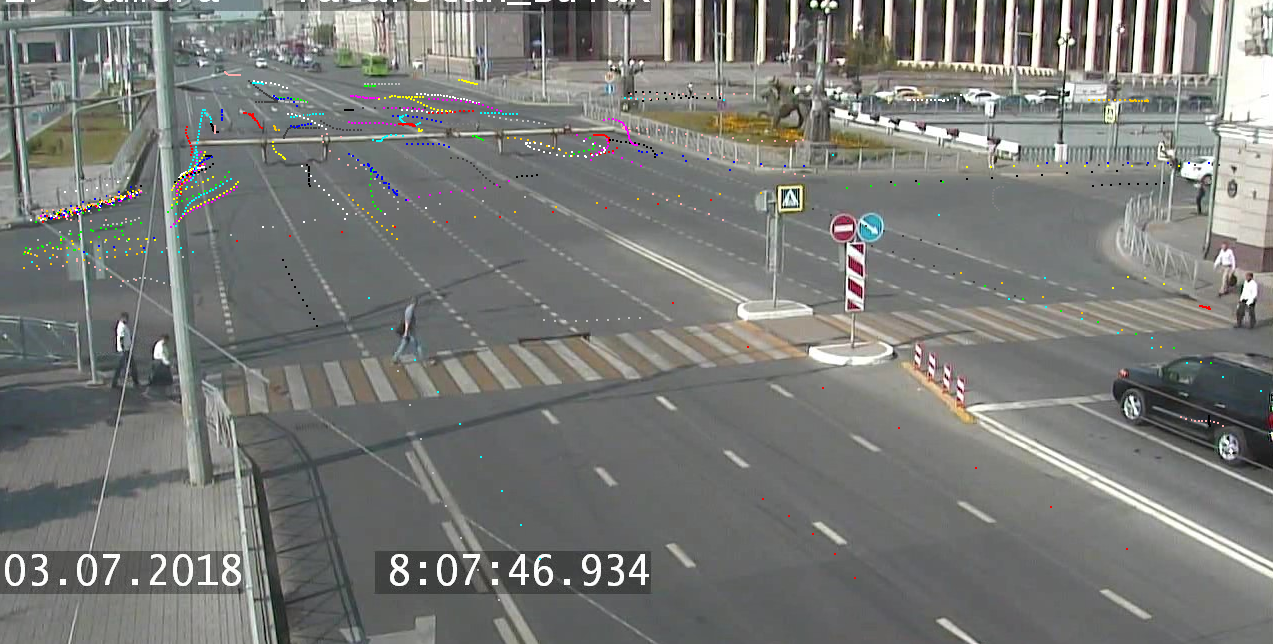
\includegraphics[width=\textwidth]{images/traj-filter-out.png}
		\caption{игнорируемые траектории}
		\label{fig:traj_filter_out}
	\end{subfigure}
	\hfill
	\begin{subfigure}[b]{0.48\textwidth}
		\centering{}
		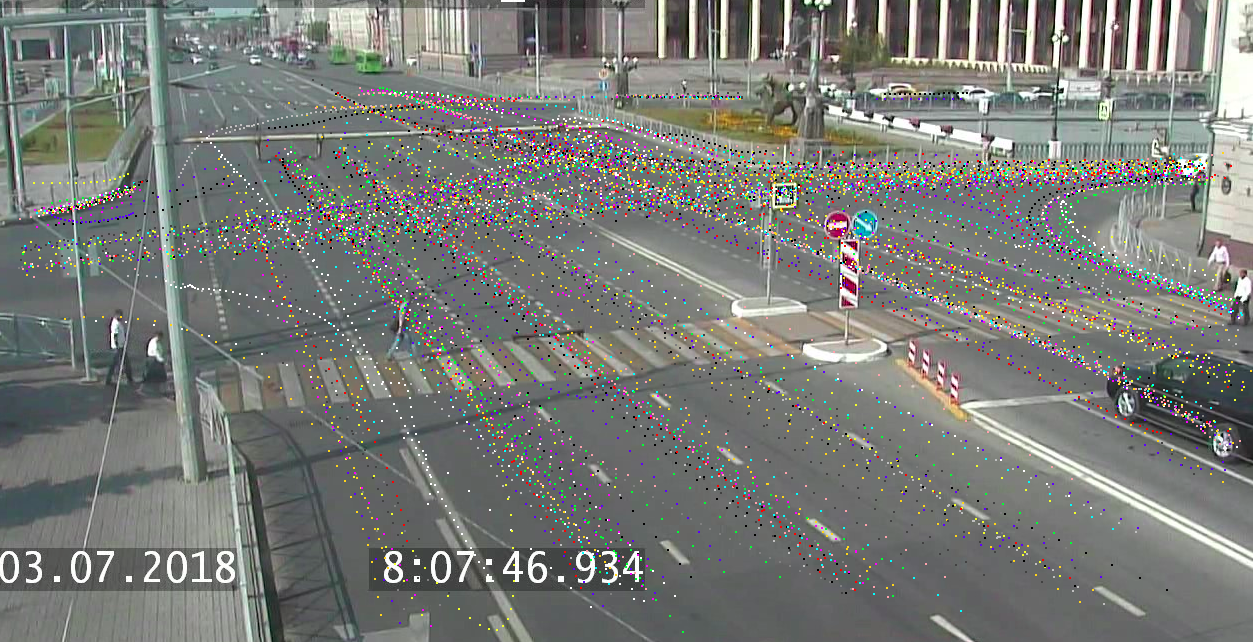
\includegraphics[width=\textwidth]{images/traj-filter-keep.png}
		\caption{оставленные траектории}
		\label{fig:traj_filter_keep}
	\end{subfigure}
	\caption{Результаты фильтрации траекторий на примере данных с первого перекрестка}
	\label{fig:traj_filter}
\end{figure}

Как уже упоминалось ранее, текущая работа сфокусирована на задаче выявления двух типов нарушений: пространственных и пространственно-временных. Для выявления аномалий первой группы достаточно проанализировать пространственную информацию о траекториях. Обнаружение аномалий второй категории, которая формируется из траекторий ТС, движущихся с аномально низкой или высокой скоростью, требует учета временной информации вместе с пространственной. По этой причине средняя постоянная скорость $\upsilon$ рассчитывается для каждой из входных траекторий $T$ в конце этапа парсинга данных как (\ref{eq:avg_speed}):

\begin{equation} \label{eq:avg_speed}
\upsilon_{avg}(T) = \frac{distance_{total}} {time_{total}},
\end{equation}

где $distance_{total}$ - итоговое пройденное расстояние между первой и последней точками траектории, а $time_{total}$ - прошедшее время. Общее расстояние может быть вычислено как сумма евклидовых расстояний между точками траектории на соседних кадрах. Поскольку известно, что кадры сняты с межкадровым интервалом 0,01 секунды, вычисление скорости может быть реализовано следующим образом (лист. \ref{lst:speed-calc}):

\lstset{style=code-style-java}
\lstinputlisting[caption={Подсчет скорости ТС}, label={lst:speed-calc}] {listings/calcSpeed.java}

\section{Аппроксимация траекторий с использованием Полиномиальной Регрессии}

Как обсуждалось ранее, полиномиальная регрессия будет использоваться для аппроксимации исходных траекторий. Были использованы готовые реализации классов-сущностей полинома\footnote{Реализация полинома \url{https://javadoc.io/doc/org.apache.commons/commons-math3/3.4.1/org/apache/commons/math3/analysis/polynomials/PolynomialFunction.html}} (необходим для дальнейшего анализа уравнений аппроксимации и поиска ключевых точек) и метода решения полиномиальных уравнений\footnote{Реализация метода решения полиномиальных функций \url{https://www.javadoc.io/doc/org.apache.commons/commons-math3/3.4.1/org/apache/commons/math3/analysis/solvers/LaguerreSolver.html}} из библиотеки Apache Commons Math 3.4.1. Для выполнения полиномиальной регрессии\footnote{Реализация полиномиальной регрессии \url{https://algs4.cs.princeton.edu/14analysis/PolynomialRegression.java}} была выбрана реализация, предоставленная авторами Р. Седжвиком и К. Уэйном для языка программирования Java \cite{online:polynomial_impl}. Все готовые к использованию реализации были пользовательскими вспомогательными методами.

Класс $PolynomialRegression$ принимает в качестве входных данных ожидаемую степень аппроксимирующего полинома ($d$) и два массива данных из N точек, состоящих из действительных чисел: массив независимых переменных ($double[]\ t$), данные о времени в данном случае, и массив зависимых переменных ($double[]\ x$, $double[]\ y$), пространственные $x$- или $y$-координаты. Затем он выполняет полиномиальную регрессию для входного набора из N точек данных $(t_i, x_i)$ или $(t_i, y_i)$ и пытается подобрать многочлен $x = \beta_0 + \beta_1 t + \beta_2 t^2 + \ldots \beta_d t^d$, где $\beta_i$ - коэффициенты регрессии, минимизирующие сумму квадратов ошибок модели полиномиальной регрессии. Поиск наилучшего решения для полиномиальных параметров основан на методе наименьших квадратов \cite{article:behav_form_extr}.

Для достижения лучшей аппроксимации оценка результатов полиномиальной регрессии выполнялась с использованием коэффициента детерминации, обозначаемого как $R^2$ (также известного как $R$-$squared$, $R$-$квадрат$ оценка, \textit{коэффициент регрессии Пирсона}) \cite{inbook:stats}. $R^2$ измеряет долю дисперсии зависимой переменной, которая может быть объяснена регрессионной моделью с заданными параметрами и является предсказуемой из независимой (объясняющей) переменной, и вычисляется следующим образом:

\begin{equation}\label{eq:r_sq}
	R^2 = 1 - \frac{SSE}{TSS} = 1 - \frac{\sum{(y_i - \hat{y_i})^2}}{\sum{(y_i - \overline{y})^2}}
\end{equation}

где $SSE$ (Sum of Squares due to Error, сумма квадратов остатков, или ошибок, регрессии) рассчитывается как сумма квадратов разностей между фактическими значениями $y_i$ и прогнозируемыми (расчетными) значениями зависимых переменных $\hat{y_i}$, и $TSS$ (Total Sum of Squares, общая сумма квадратов) рассчитывается как сумма квадратов отклонений фактического значения $y_i$ от среднего значения $\overline{y}$.

Коэффициент $R^2$ может принимать значения между [0, 1], где близкое к 1 значение указывает на то, что существует сильная зависимость меду выбранными параметрами и модель (в данном случае полиномиальное уравнение) отлично предсказывает данные \cite{online:reg_r_interpr}. Модели со значением коэффициента выше 0,8 принято считать адекватными, значение 1 свидетельствует о наличии функциональной зависимости между переменными.

В этой работе полиномиальная регрессия была выполнена для всех исходных траекторий (Приложение B). Полученные регрессионные модели сравнивались по показателям $R^2$, результаты анализировались относительно формы и скорости траекторий. Демонстрация, сравнение и обсуждение полученных результатов представлены в следующей главе.

\subsection{Выбор ключевых точек в аппроксимированных траекториях}

Главной целью и причиной использования аппроксимированных траекторий вместо исходных для дальнейшего анализа было уменьшение сложности подсчета LCSS метрики. По этой причине длина траекторий должна быть уменьшена путем выбора нескольких ключевых репрезентативных точек из аппроксимированных траекторий путем анализа полиномов аппроксимации.

Из математики известно, что критическими точкам полинома $f(t)$ являются точки, где полиномиальная функция не дифференцируема или производная в этой точке равна нулю (стационарные точки). Стационарные точки, включая локальные минимумы и максимумы, восходящие и нисходящие точки перегиба можно найти путем анализа производных функции. Стационарные точки являются решениями уравнения, в котором первая производная функции приравнена нулю: $f'(t) = 0$. Точки перегиба могут быть найдены путем дальнейшего анализа второй производной: они соответствуют решениям уравнения $f''(t) = 0$. Для решения полиномиальных уравнений использовались готовые релизации метдов решения полиномиальных уравнений из библиотеки Apache Commons Math: $LaguerreSolver$, $BisectionSolver$ со следующими входными параметрами:

\begin{itemize}
	\item $maxItem = 30000$ -- задает максимально допустимое количество итераций в ходе поиска решения полиномиального уравнения,
	\item $min = firstTimePoint$ -- определяет нижнюю границу допустимых значений решения;
	\item $max = lastTimePoint$ -- определяет верхнюю границу допустимых значений решения;
	\item $startValue = min + 1$ -- задает начальную точку для метода решения уравнения, чтобы начать поиск решения.
\end{itemize}

Программа решения уравнений вызывалась для полиномиальных функций, полученных как первая и вторая производные, взятые из полиномов для $X$- и $Y$-координат. Вызов метода решения приведен в лист. \ref{lst:solver-init}:

\lstinputlisting[caption={Вызов метода решения полиномиальных уравнений}, label={lst:solver-init}] {listings/initSolver.java}

Решения, найденные двумя методами, объединяются: остаются только точки, относящиеся к разным точкам времени.

В случае анализа траекторий точки перегиба очень значимы и репрезентативны, поскольку они несут важную информацию о форме траектории: ключевые точки обозначают места основных поворотов или изменения траектории.

Однако критические точки не всегда могут быть найдены из-за вычислительных ограничений полиномиальных функций высокого порядка. Следовательно, критических точек, идентифицированных таким образом, недостаточно, чтобы полностью описать поведение исходной траектории и использовать для дальнейшего анализа, поскольку они не предоставляют всей информации о границах формы траектории и не всегда могут отобразить все повороты. По этой причине было решено добавить граничные для траектории ключевые точки, взяв отдельно минимальные и максимальные координаты $X$ и $Y$ и вычислив соответствующие точки траектории с использованием соответствующей регрессионной модели (лист. \ref{lst:key-borders-calc}).

\lstinputlisting[caption={Вычисление граничных ключевых точек траектории}, label={lst:key-borders-calc}] {listings/calcKeyBorders.java}

Результаты аппроксимации полиномиальной регрессией и вычисления ключевых точек представлены на рисунке \ref{fig:regr-kp}. Точки траектории, относящиеся к исходным данным траектории, изображены с использованием красного цвета, тогда как синие точки траектории соответствуют точкам, полученным с использованием функций полиномиального приближения для тех же временных точек. Ключевые точки каждой траектории выделены жирными синими квадратными точками. Видно, что функция аппроксимации близка к исходной функции траектории, для некоторых траекторий приближение дает те же координаты, что и в исходных данных (для траекторий с полиномами аппроксимации, имеющими $R^2 \approx 1.0$). Также можно заметить, что ключевые точки точно придерживаются линии аппроксимации и правильно описывают траекторию, следовательно, они могут использоваться вместо исходных точек траектории для упрощения дальнейшего анализа траекторий.

\begin{figure}[!htb]
	\centering
	\begin{subfigure}[!htb]{0.68\textwidth}
		\centering{}
		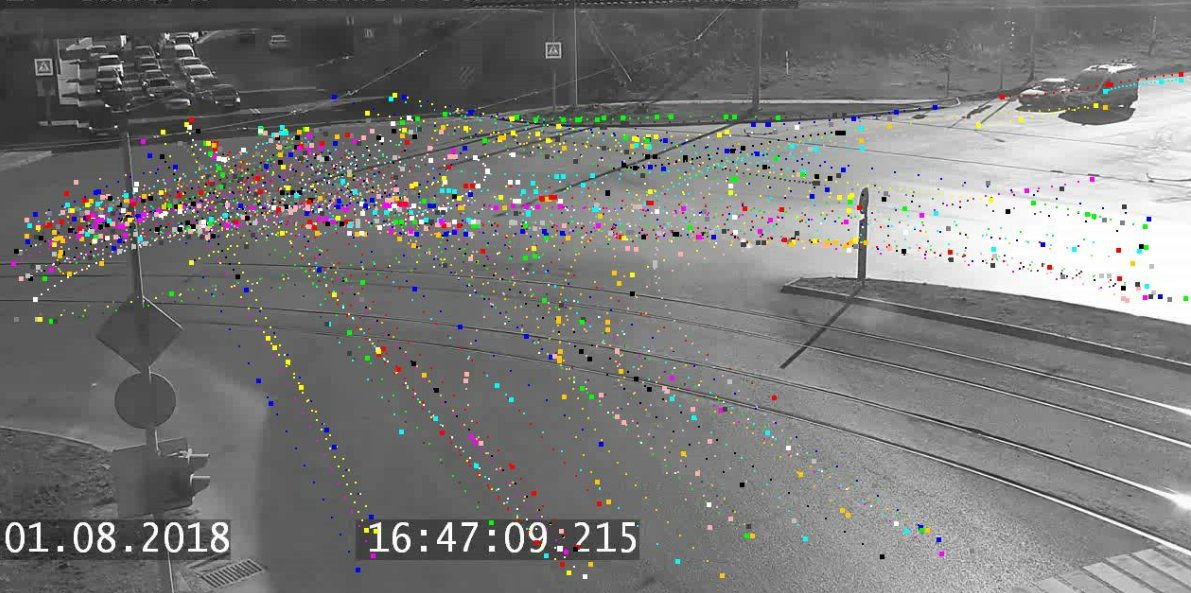
\includegraphics[width=\textwidth]{images/regr_kp_full.png}
		\caption{множество всех исходных траекторий $2.txt$}
	\end{subfigure}
	\hfill
	\begin{subfigure}[!htb]{0.3\textwidth}
		\centering{}
		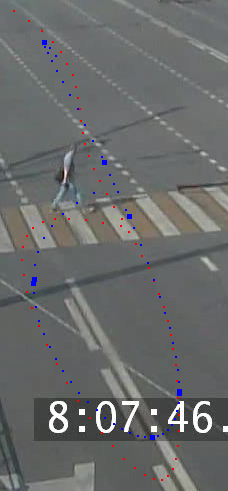
\includegraphics[width=\textwidth]{images/regr_kp_loop.png}
		\caption{траектория-петля $1.txt$}
	\end{subfigure}
	\hfill
	\begin{subfigure}[!htb]{0.3\textwidth}
		\centering{}
		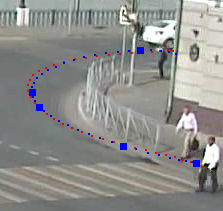
\includegraphics[width=\textwidth]{images/regr_kp_turn.png}
		\caption{траектория с поворотом $1.txt$}
	\end{subfigure}
	\hfill
	\begin{subfigure}[!htb]{0.3\textwidth}
		\centering{}
		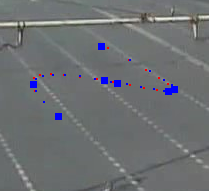
\includegraphics[width=\textwidth]{images/regr_kp_complex.png}
		\caption{траектория сложной формы $1.txt$}
	\end{subfigure}
	\hfill
	\begin{subfigure}[!htb]{0.3\textwidth}
		\centering{}
		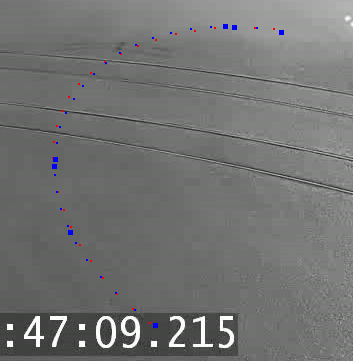
\includegraphics[width=\textwidth]{images/regr_kp_curve_2.png}
		\caption{изогнутая траектория $2.txt$}
	\end{subfigure}
	\hfill
	\begin{subfigure}[!htb]{0.3\textwidth}
		\centering{}
		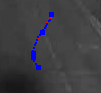
\includegraphics[width=\textwidth]{images/regr_kp_complex_3.png}
		\caption{траектория сложной формы $3.txt$}
	\end{subfigure}
	\hfill
	\begin{subfigure}[!htb]{0.3\textwidth}
		\centering{}
		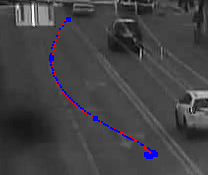
\includegraphics[width=\textwidth]{images/regr_kp_curve_3.png}
		\caption{изогнутая траектория $3.txt$}
	\end{subfigure}
	\hfill
	\begin{subfigure}[!htb]{0.3\textwidth}
		\centering{}
		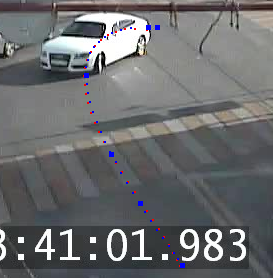
\includegraphics[width=\textwidth]{images/regr_kp_curve_4.png}
		\caption{траектория-поворот $4.txt$}
	\end{subfigure}

	\caption{Результаты полиномиальной регрессии с обозначением ключевых точек}
	\label{fig:regr-kp}
\end{figure}

\section{Вычисление метрики схожести траекторий}

Как упоминалось ранее, LCSS метрика будет использоваться в качестве метрики для измерения сходства между траекториями. Следовательно, расстояние LCSS (метрика различия) будет рассчитываться на основе метрики сходства LCSS в соответствии с вышеупомянутыми формулами. Стоит отметить, что LCSS метрика является симметричной и для пары траекторий может быть вычислена только один раз \cite{inproceedings:28_lcss_dsmt}.

Несмотря на то что реализация LCSS метрики присутствует в пакете R \cite{online:r_lcss}, представленная реализация не позволяет использование динамических, адаптивных параметров $\delta$ и $\varepsilon$. По этой причине в рамках реализации фреймворка была написан пользовательская реализация метода подсчета LCSS метрики, представленный в лист. \ref{lst:lcss-calc}.

\lstinputlisting[caption={Вычисление LCSS}, label={lst:lcss-calc}] {listings/calcLCSS.java}

\section{Кластеризация}

Поскольку не было найдено подходящей реализации иерархической кластеризации для траекторий с использованием расстояния LCSS и возможностью обрабатывать адаптивные значения параметров, кластеризация, а также вычисление метрики LCSS, были написаны с нуля. Реализация была написана на основе алгоритма \ref{algo:ahc-descr}, представленного выше, в общих чертах описывающего алгоритм. Исходный код кластеризации приведен в Приложении С.

Кластеризация выполняется итеративно методом последовательного объединения двух ближайших кластеров в один с последующим пересчетом матрицы подобия (близости) кластеров. Метод кластеризации принимает в качестве входных данных параметр $OUTPUT\_CLUSTERS\_COUNT$, который определяет ожидаемое итоговое количество кластеров. Если полученное значение пустое ($null$), оно будет рассматриваться как 1, и кластеризация будет выполняться до тех пор, пока все кластеры не будут объединены в один в соответствии с базовым алгоритмом агломеративной иерархической кластеризации, или пока дальнейшее объединение кластеров будет невозможно.

\subsection{Моделирование кластеров}

Clusters modeling implementation		% Framework
\chapter{Результаты}
\label{ch:Результаты}

В этой главе описываются оценочные тесты, выполненные для проверки предложенного подхода на основе разработанного фреймворка. Следующие разделы предназначены для предоставления информации о подготовке исходных данных, представления и обсуждения полученных результатов. Сначала будет рассмотрена аппроксимация траекторий с использованием полиномиальной регрессии. Далее будет проведена провека точности результирующих кластеров точность с использованием вышеупомянутого индекса DI. Глава завершается обсуждением выходных результатов этапа классификации и демонстрацией результатов проверки качества обнаружения аномалий.

\section{Оценка точности}

В этом разделе подробно описываются подготовка и результаты оценочных тестов, выполненных для проверки точности, достоверности полученных результатов.

\subsection{Результаты аппроксимации траекторий}

Для того чтобы принять решение о степени полиномов для аппроксимации, было проведено несколько экспериментов. Были предприняты попытки аппроксимировать исходные траектории полиномами $3$-ей, $4$-ой, $5$-ой степеней соответственно. В следующей таблице приведены минимальные и средние значения коэффициента детерминации $R^2$ для каждого из экспериментов (табл. \ref{table:r2_res}).

\begin{table}[h!]
	\caption{Значения коэффициента $R^2$ для полиномов различных степеней}
	\label{table:r2_res}
	
	\setlength{\tabcolsep}{10pt}
	\centering
	\begin{tabular}[c]{|| C{2cm} | C{2cm} C{2cm} | C{2cm} C{2cm} ||} 
		\hline
		\multirow{3}{7em}{Degrees of polynomials} 	& \multicolumn{4}{c||}{$R^2$ score} \\[1ex]\cline{2-5}
		& \multicolumn{2}{c|}{X}	& \multicolumn{2}{c||}{Y} \\ [0.5ex]
		& min 	& avg				& min 	& avg \\ [0.5ex]
		\hline \hline
		\rowcolor{nogray} \multicolumn{5}{||c||}{$1.txt$ (before filtering)} \\ [0.5ex]
		\hline
		\{3\} 							& 0.66 	& 0.994 & 0.466 & 0.989 \\ [2ex]
		\rowcolor{backgray} \{3, 4\} 	& 0.897 & 0.998 & 0.823 & 0.994 \\ [2ex]
		\{3, 4, 5\} 					& 0.949 & 0.998 & 0.864 & 0.995 \\ [2ex]
		
		\hline \hline
		\rowcolor{nogray} \multicolumn{5}{||c||}{$1.txt$} \\ [0.5ex]
		\hline
		\{3\} 							& 0.689 & 0.997 & 0.777 & 0.995 \\ [2ex]
		\rowcolor{backgray} \{3, 4\} 	& 0.942 & 0.999 & 0.872 & 0.997 \\ [2ex]
		\{3, 4, 5\} 					& 0.98 	& 0.999 & 0.88 	& 0.997 \\ [2ex]
		
		\hline \hline
		\rowcolor{nogray} \multicolumn{5}{||c||}{$2.txt$} \\ [0.5ex]
		\hline
		\{3, 4\} 						& 0.992 & 0.9997 & 0.832 & 0.996 \\ [2ex]
		\hline \hline
		
		\rowcolor{nogray} \multicolumn{5}{||c||}{$3.txt$} \\ [0.5ex]
		\hline
		\{3, 4\} 						& 0.815 & 0.995 & 0.867 & 0.996 \\ [2ex]
		\hline \hline
		
		\rowcolor{nogray} \multicolumn{5}{||c||}{$4.txt$} \\ [0.5ex]
		\hline
		\{3, 4\} 						& 0.879 & 0.995 & 0.722 & 0.993 \\ [2ex]
		\hline
	\end{tabular}
\end{table}

В этом параграфе будет приведено обсуждение результатов экспериментов на примере траекторий с первого перекрестка ($ 1.txt $) до и после фильтрации траекторий. Из табл. \ref{table:r2_res} видно, что средние значения коэффициента $R^2$ приемлемы для всех экспериментов. Однако минимальные значения $R^2$, которые равны 0,66 и 0,466 для первого эксперимента с полиномами только $3$-ей степени для неотфильтрованных траекторий являются неудовлетворительными, что означает, что модель может корректно предсказать только половину всех точек траекторий. Фильтрация и игнорирование коротких траекторий с малым итоговым пространственным смещением значительно улучшили результаты. Однако результаты для аппроксимации с использованием полиномов $3$-ей степени все еще неудовлетворительны. Это может повлиять на последующий анализ и ухудшить дальнейший анализ. По этой причине было выполнено приближение с использованием полиномов различных степеней одновременно следующим образом:

\begin{enumerate}
	\item сначала выполнить аппроксимацию, используя низшую степень полинома в качестве отправной точки,
	\item сравнить полученные значения коэффициента детерминации $R^2$ с заранее заданным граничным значением (0,98 в данном случае); если полученное значение меньше предопределенного порога, увеличить ожидаемую степень полинома и выполнить полиномиальную регрессию снова,
	\item продолжать увеличивать степень полинома до получения приемлемых значений $R^2$ или до достижения заданного ограничения максимальной допустимой степени полинома (5 в данном случае). 
\end{enumerate} 

Аппроксимация полиномами $3$-ей и $4$-ой степеней в совокупности значительно улучшила как минимальные, так и средние значения $R^2$. Однако добавление полинома $5$-ой степени не оказало существенного влияния на результаты и улучшило средний коэффициент только на 0,01 по сравнению с предыдущим экспериментом. В связи с этим было решено сосредоточиться на приближении с использованием полиномиальных функций $3$-ей и $4$-ой степеней и провести эксперименты на траекториях с других перекрестков ($2.txt$, $3.txt$, $4.txt$).

Для упрощения повествования траектории будут классифицированы на две группы в зависимости от степени полиномов, использованных для аппроксимации: первая группа включает в себя траектории, аппроксимированные полиномиальными функциями $3$-ей степени, в то время как вторая группа состоит из траекторий, аппроксимируемых полиномами $4$-ой степени. Траектории обеих групп были проанализированы с точки зрения формы и средней скорости. На рис. \ref{fig:regr-pol-4} показана вторая группа траекторий, а в табл. \ref{table:speeds} указаны представлены минимальная, средняя и максимальная скорости траекторий для обеих групп.

\begin{figure}
	\centering
	\begin{subfigure}[b]{0.3\textwidth}
		\centering{}
		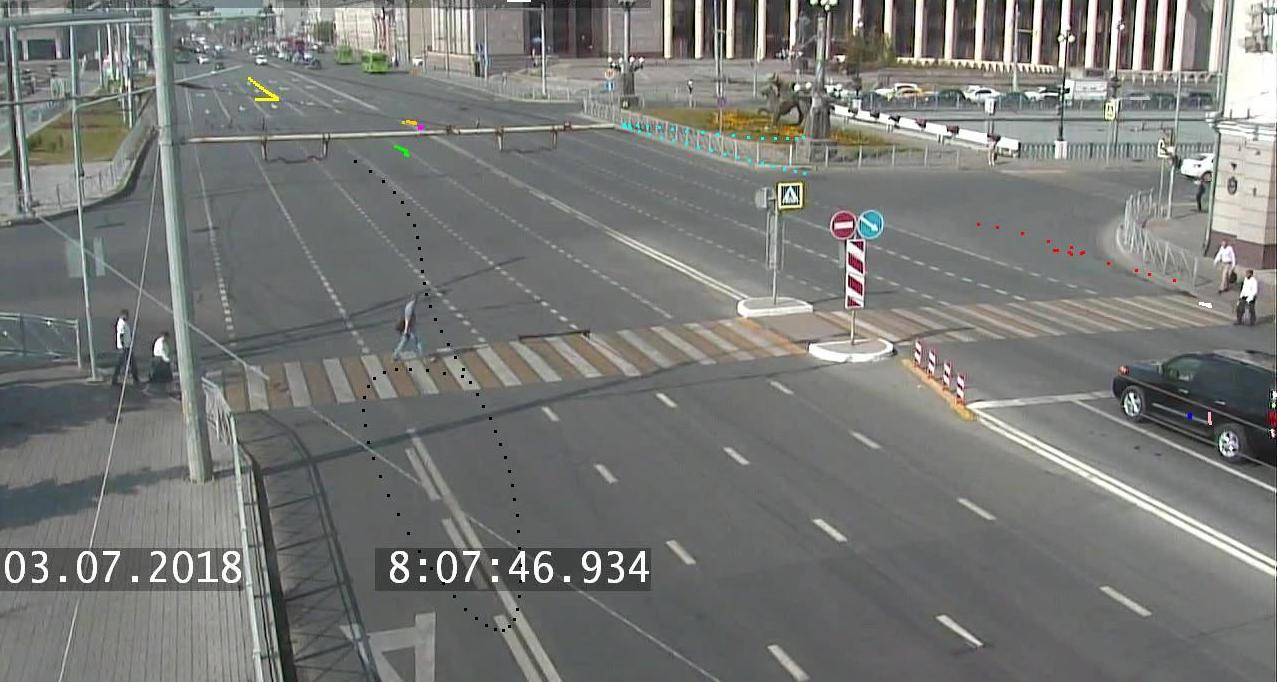
\includegraphics[width=\textwidth]{images/regr_1_pol_4.jpg}
		\caption{$1.txt$}
		\label{fig:regr-1-pol-4}
	\end{subfigure}
	\hfill
	\begin{subfigure}[b]{0.3\textwidth}
		\centering{}
		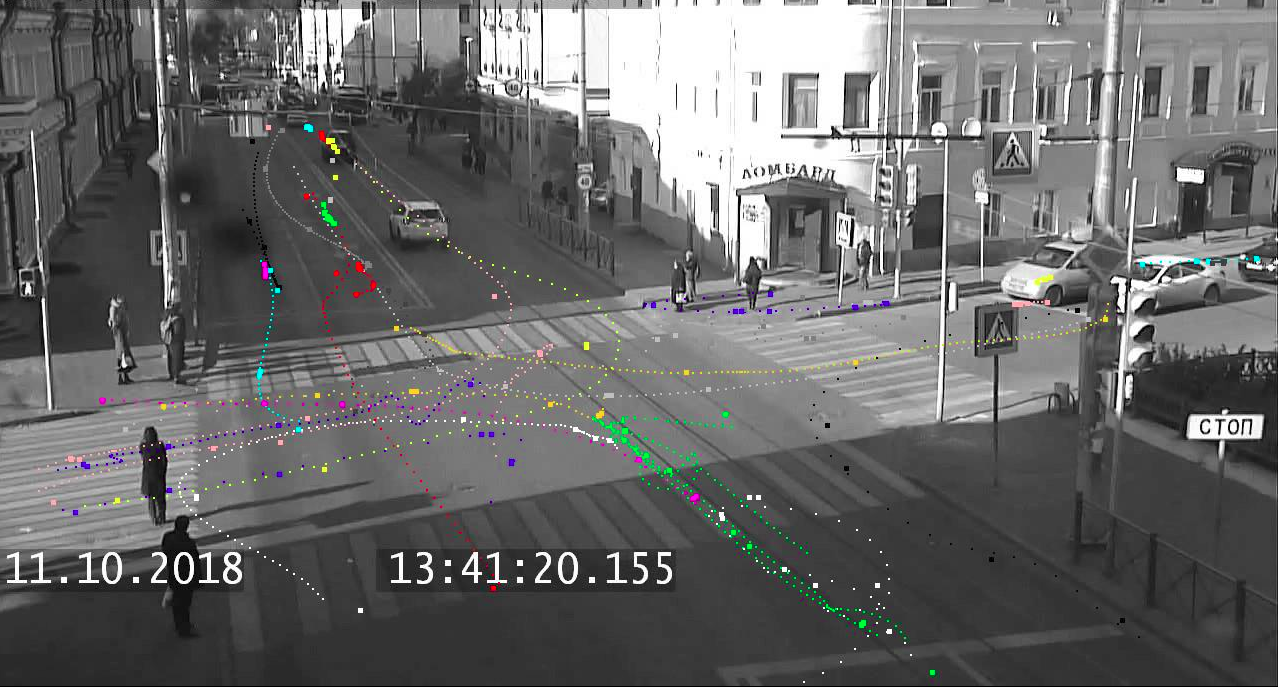
\includegraphics[width=\textwidth]{images/regr_3_pol_4.png}
		\caption{$3.txt$}
		\label{fig:regr-3-pol-4}
	\end{subfigure}
	\hfill
	\begin{subfigure}[b]{0.3\textwidth}
		\centering{}
		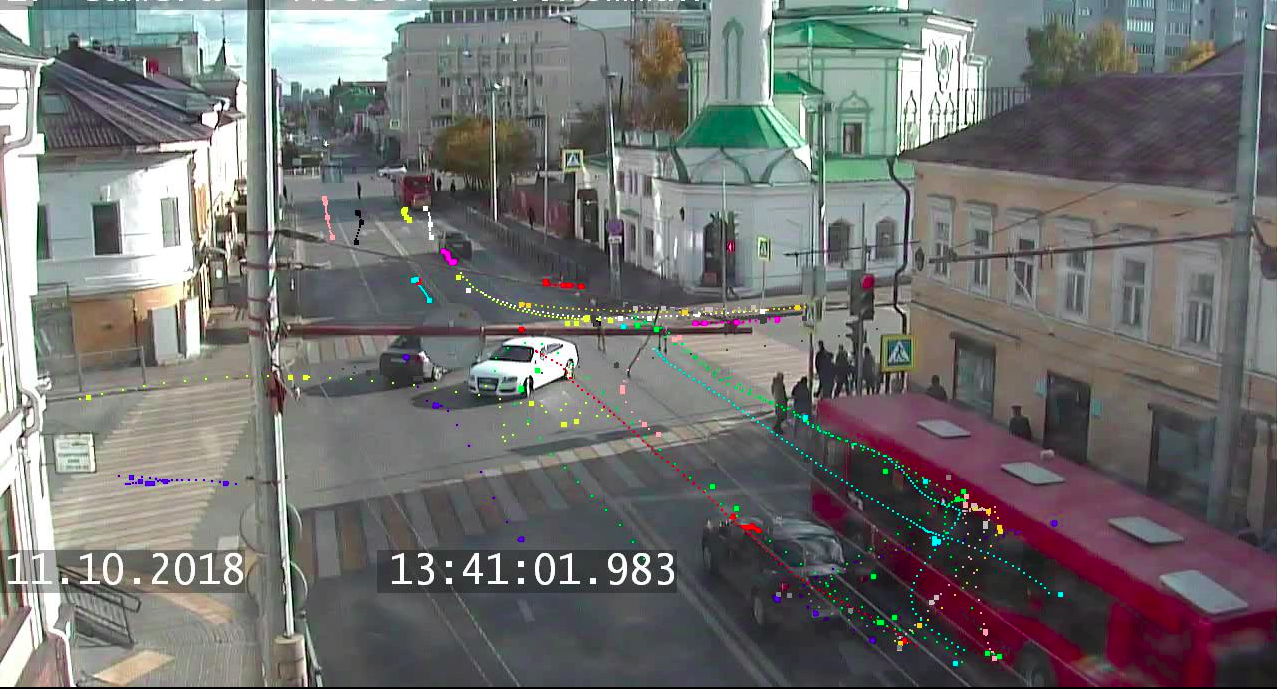
\includegraphics[width=\textwidth]{images/regr_4_pol_4.png}
		\caption{$4.txt$}
		\label{fig:regr-4-pol-4}
	\end{subfigure}
	\caption{Траектории, аппроксимированные полиномами $4$-ой степени}
	\label{fig:regr-pol-4}
\end{figure}

\begin{table}[h!]
	\caption{Сравнение минимальной, средней, максимальной скоростей ТС}
	\label{table:speeds}
	
	\setlength{\tabcolsep}{10pt}
	\centering
	\begin{tabular}[c]{|| C{2.5cm} | C{2.5cm} C{2.5cm} C{2.5cm} ||} 
		\hline
		\multirow{2}{7em}{Degree of a polynomial} 	
		& \multicolumn{3}{c||}{Speed \textit{(pixels per sec)}} \\[1ex]\cline{2-4}
		& min 		& avg		& max 				\\ [2ex]
		
		\hline \hline
		\rowcolor{nogray} \multicolumn{4}{||c||}{$1.txt$ (before filtering)} 	\\ [0.5ex]
		\hline
		\rowcolor{backgray} \{3\} 	& 18.555 	& 335.365 	& 1721.499 			\\ [2ex]
		
		\rowcolor{backgray} \{4\} 	& 1.206		& 72.34 	& 374.396 			\\ [2ex]
		\hline
		
		\rowcolor{nogray} \multicolumn{4}{||c||}{$1.txt$} 	\\ [0.5ex]
		\hline
		\rowcolor{backgray} \{3\} 	& 61.814 	& 372.435 	& 909.121 			\\ [2ex]
		
		\rowcolor{backgray} \{4\} 	& 26.603	& 229.053 	& 602.773 			\\ [2ex]
		
		\hline
		\rowcolor{nogray} \multicolumn{4}{||c||}{$2.txt$} 	\\ [0.5ex]
		\hline
		\{3\} 	& 85.705 	& 494.016 	& 1107.96 			\\ [2ex]
		
		\{4\} 	& 183.087	& 613.865 	& 900.737 			\\ [2ex]
		\hline
		
		\rowcolor{nogray} \multicolumn{4}{||c||}{$3.txt$} 	\\ [0.5ex]
		\hline
		\{3\} 	& 13.65 	& 301.481 	& 1012.748 			\\ [2ex]
		
		\{4\} 	& 29.26		& 206.119 	& 764.25 			\\ [2ex]
		\hline
		
		\rowcolor{nogray} \multicolumn{4}{||c||}{$4.txt$} 	\\ [0.5ex]
		\hline
		\{3\} 	& 43.01 	& 269.074 	& 872.33	 		\\ [2ex]
		
		\{4\} 	& 22.92		& 163.431 	& 708.154 			\\ [2ex]
		\hline
		
	\end{tabular}
\end{table}

Далее траектории, аппроксимированные полиномами $3$-ей $4$-ой степеней будут обозначаться первой и второй группами траекторий соответственно. Можно заметить, что траектории из разных групп имеют очень разные скорости. Первая группа включает в себя траектории с гораздо более высокими скоростями, особенно выделяется, что максимальная скорость для второй группы почти равна средней скорости для первой группы, а средняя скорость для первой группы почти в четыре раза больше, чем для второй группы для случая неотфильтрованных траекторий. После исключения коротких траекторий из рассмотрения результаты стали более плавными, однако те же наблюдения и выводы имеют место быть. Также на рис. \ref{fig:regr-pol-4} видно, что полиномиальные функции 4-го порядка использовались для аппроксимации траекторий более сложной формы или траекторий с плотно расположенными точками траектории.

Такая тенденция в основном различима при рассмотрении траекторий с первого перекрестка. Данные с первого перекрестка могут считаться репрезентативным набором траекторий, поскольку он имеет наибольшее количество экземпляров данных. Также стоит отметить, что второй набор данных траекторий ($2.txt$) имеет только 10 траекторий в первой группе, поэтому анализ скорости траекторий не может быть очень точным.

\subsubsection{Выводы}

Таким образом, из вышеизложенных результатов следует, что полиномиальные функции высшего порядка предпочтительнее для аппроксимации траекторий следующих групп:

\begin{itemize}
	\item траектории медленно движущихся или неактивных ТС (включая траектории ТС, ожидающих на перекрестках на светофоре), которые продемонстрированы на \ref{fig:regr-1-pol-4};
	\item траектории ТС, движущихся с непостоянной скоростью или ускорением на некоторых участках траектории (могут быть представлены неравным распределением точек траектории, где плотные области точек траектории сигнализируют об ускорении в течение этих временных интервалов; как результат, полиномы низкого порядка не могут описать такую сложную зависимость между пространственной координатой и временем);
	\item траектории сложной формы (резкие повороты, улитки Паскаля), особенно различимо на рис. \ref{fig:regr-pol-4}b-c.
\end{itemize}

\subsection{Результаты кластеризации траекторий} 		% Evaluation and Experiments
\chapter{ЗАКЛЮЧЕНИЕ}
\label{ch:ЗАКЛЮЧЕНИЕ}

В этой работе был предложен и проанализирован подход для идентификации траекторных аномалий в неопределенных пространственно-временных данных. Для оценки и реализации подхода была разработан фреймворк, решающий поставленную задачу. Исходный код реализации доступен в репозитории GitHub \cite{online:mt_anomalies}. Для решения задачи обнаружения аномалий в качестве основы использовался кластерный подход, а именно алгоритм агломеративной иерархической кластеризации. Для вычисления меры сходства и различия между траекториями и кластерами была выбрана и реализована метрика расстояния LCSS. Однако, как было упомянуто в предыдущих главах, вычисление расстояния LCSS по классическому алгоритму становится невозможным для длинных траекторий. По этой причине была выполнена аппроксимация входных траекторий с использованием полиномиальной регрессии. Согласно результатам оценки, наилучшая точность аппроксимации достигается при совместном использовании полиномиальных функций $3$-ей и $4$-ой степеней. Таким образом, кластеризация была выполнена на отфильтрованном наборе приближенных входных траекторий с использованием отобранных ключевых точек для каждой из них. Точность выполненной кластеризации была оценена с использованием индекса DI и равна $0,95$, что говорит о качественном разделении на четкие различимые кластеры.

В результате данной работы можно сделать следущие выводы:
\begin{itemize}
	\item аппроксимация коротких траекторий с непостоянной скоростью требует использования полиномиальных функций более высоких степеней,
	\item несмотря на то что LCSS метрика расстояния позволяет траекториям быть разной длины, ее вычисление становится чрезвычайно трудоемким и времязатратным  для траекторий с более чем 11-12 точками траекторий,
	\item аппроксимация траекторий с использованием полиномиальной регрессии дает точные результаты, поскольку заранее известно, что существует функционлаьная зависимость между пространственными координатами траектории и временным параметром (согласно принципам физики, скорости, ускорения и т.д.).
	
\end{itemize}

\bigbreak

\subsubsection{Дальнейшее развитие}

Предложенный подход и разработанный фреймворк спроектированы в манере обучения оффлайн что означает, что модели поведения нормальных и аномальных траекторий изучаются и запоминаются заранее и не обновлятся впоследствии. Последующие исследования могут включать изучение возможности обновления базы данных нормальных траекторий по мере поступления новых данных, чтобы сделать подход и сам фреймворк адаптирующимся к реальным актуальным данным транспортного трафика.
 		% Conclusion and Perspectives

% Bibliography
%\bibliography{bibliography}
\clearpage

\listoffigures
\clearpage
\listoftables

\renewcommand{\listalgorithmcfname}{Алгоритмы}
\listofalgorithms
\addcontentsline{toc}{chapter}{Список алгоритмов}

\begingroup
\let\clearpage\relax
\lstlistoflistings
\endgroup
\addcontentsline{toc}{chapter}{Список листингов}
\clearpage

\pagenumbering{Roman}
%%%%%%%%%%%END%%%%%%%%%%%

%\appendix
\section*{ПРИЛОЖЕНИЕ}
\markboth{ПРИЛОЖЕНИЕ}{ПРИЛОЖЕНИЕ}
\addcontentsline{toc}{chapter}{ПРИЛОЖЕНИЕ}

\subsection*{A. Алгоритм парсинга входных траекторий}
\addcontentsline{toc}{section}{A. Алгоритм парсинга входных траекторий}
\lstset{style=code-style-java}
\lstinputlisting[caption={Алгоритм парсинга входных траекторий}, label={lst:parse-traj}] {listings/parsing.java}

\subsection*{B. Инициирование Полиномиальной Регрессии}
\addcontentsline{toc}{section}{B. Инициирование Полиномиальной Регрессии}
\lstinputlisting[caption={Инициирование полиномиальной регрессии}, label={lst:pol-regr}] {listings/polRegr.java}

\subsection*{C. Агломеративная Иерархическая Кластеризация}
\addcontentsline{toc}{section}{C. Агломеративная Иерархическая Кластеризация}
\lstinputlisting[caption={Реализация кластеризации}, label={lst:clust-impl}] {listings/clustImpl.java}


\end{document}
%%% Конец документа